% Para utilizar este template siga o tutorial disponível em http://www.biblioteca.ufc.br/images/arquivos/instrucoes_modelos/tutorial_sharelatex.pdf

%%%%%%%%%%%%%%%%%%%%%%%%%%%%%%%%%%%%%%%%%%%%%%%%%%%%%%%
%% Você dever criar uma conta no ShareLatex. Depois, %%
%% vá nas opções no canto esquerdo superior da tela  %%
%% e clique em "Copiar Projeto". Dê um novo nome pa- %%
%% ra o projeto.                                     %%
%%                                                   %%
%% Os principais desenvolvedores deste template são: %%
%%                                                   %%
%%            Ednardo Moreira Rodrigues              %%
%%     (Doutorando em Engenharia Elétrica - UFC)     %%
%%                      &                            %%
%%            Alan Batista de Oliveira               %%
%%     (Graduando em Engenharia Elétrica - UFC)      %%
%%                                                   %%
%% Revisão:                                          %%
%%                                                   %%
%% - Eliene Maria Vieira de Moura;                   %%
%% - Francisco Edvander Pires Santos;                %%
%% - Izabel Lima dos Santos;                         %%
%% - Juliana Soares Lima;                            %%
%% - Kalline Yasmin Soares Feitosa.                  %%
%%                                                   %%
%% Colaborador:                                      %%
%% -Andrei Bosco Bezerra Torres                      %% 
%% (Professor - Sistemas e Mídias Digitais -         %%
%% Instituto Universidade Virtual - UFC)             %%
%%                                                   %%
%% Grande parte do trabalho foi adaptado do template %%
%% da UECE elaborado por:                            %%
%% Thiago Nascimento  (UECE)                         %%
%% Project available on:                             %%
%% https://github.com/thiagodnf/uecetex2             %%
%%                                                   %%
%% "Dúvidas, esclarecimentos ou sugestões podem ser  %%
%% enviadas para o e-mail da Comissão de Serviços da %%
%% Biblioteca Universitária: csbu@ufc.br."           %%
%%                                                   %%
%% As últimas atualizações estão descritas no inicio %%
%% do arquivo "README.md".                           %%
%%                                                   %%
%%%%%%%%%%%%%%%%%%%%%%%%%%%%%%%%%%%%%%%%%%%%%%%%%%%%%%%

\documentclass[        
    a4paper,          % Tamanho da folha A4
    12pt,             % Tamanho da fonte 12pt
    chapter=TITLE,    % Todos os capitulos devem ter caixa alta
    section=Title,    % Todas as secoes devem ter caixa alta somente na primeira letra
    subsection=Title, % Todas as subsecoes devem ter caixa alta somente na primeira letra
    oneside,          % Usada para impressao em apenas uma face do papel
    english,          % Hifenizacoes em ingles
    spanish,          % Hifenizacoes em espanhol
    brazil,           % Ultimo idioma eh o idioma padrao do documento
    fleqn             % Coloca as equações alinhadas a esquerda
]{abntex2}


% Para utilizar este template siga o tutorial disponível em http://www.biblioteca.ufc.br/images/arquivos/instrucoes_modelos/tutorial_sharelatex.pdf

%%%%%%%%%%%%%%%%%%%%%%%%%%%%%%%%%%%%%%%%%%%%%%%%%%%%%%%
%%      Para começar a usar este template, primeiro, %%
%% você dever criar uma conta no ShareLatex. Depois, %%
%% vá nas opções no canto esquerdo superior da tela  %%
%% e clique em "Copiar Projeto". Dê um novo nome pa- %%
%% ra o projeto.                                     %%
%%                                                   %%
%% Os principais desenvolvedores deste template são: %%
%%                                                   %%
%%             Ednardo Moreira Rodrigues             %%
%%     (Doutorando em Engenharia Elétrica - UFC)     %%
%%                      &                            %%
%%            Alan Batista de Oliveira               %%
%%     (Graduando em Engenharia Elétrica - UFC)      %%
%%                                                   %%
%% Revisão:                                          %%
%%                                                   %%
%% - Eliene Maria Vieira de Moura;                   %%
%% - Francisco Edvander Pires Santos;                %%
%% - Izabel Lima dos Santos;                         %%
%% - Juliana Soares Lima;                            %%
%% - Kalline Yasmin Soares Feitosa.                  %%
%%                                                   %%
%% Grande parte do trabalho foi adaptado do template %%
%% da UECE elaborado por:                            %%
%% Thiago Nascimento  (UECE)                         %%
%% Project available on:                             %%
%% https://github.com/thiagodnf/uecetex2             %%
%%                                                   %%
%% "Dúvidas, esclarecimentos ou sugestões podem ser  %%
%% enviadas para o e-mail da Comissão de Serviços da %%
%% Biblioteca Universitária: csbu@ufc.br."           %%
%%                                                   %%
%%%%%%%%%%%%%%%%%%%%%%%%%%%%%%%%%%%%%%%%%%%%%%%%%%%%%%%

% Importações de pacotes
\usepackage[utf8]{inputenc}                         % Acentuação direta
\usepackage[T1]{fontenc}                            % Codificação da fonte em 8 bits
\usepackage{graphicx}                               % Inserir figuras
\usepackage{amsfonts, amssymb, amsmath}             % Fonte e símbolos matemáticos
\usepackage{booktabs}                               % Comandos para tabelas
\usepackage{verbatim}                               % Texto é interpretado como escrito no documento
\usepackage{multirow, array}                        % Múltiplas linhas e colunas em tabelas
\usepackage{indentfirst}                            % Endenta o primeiro parágrafo de cada seção.
\usepackage{listings}                               % Utilizar codigo fonte no documento
\usepackage{xcolor}
\usepackage{microtype}                              % Para melhorias de justificação?
\usepackage[portuguese,ruled,lined]{algorithm2e}    % Escrever algoritmos
\usepackage{algorithmic}                            % Criar Algoritmos  
%\usepackage{float}                                 % Utilizado para criação de floats
\usepackage{amsgen}
\usepackage{lipsum}                                 % Usar a simulação de texto Lorem Ipsum
%\usepackage{titlesec}                              % Permite alterar os títulos do documento
\usepackage{tocloft}                                % Permite alterar a formatação do Sumário
\usepackage{etoolbox}                               % Usado para alterar a fonte da Section no Sumário
\usepackage[nogroupskip,nonumberlist]{glossaries}   % Permite fazer o glossario

\usepackage[font=singlespacing,format=plain,justification=justified,skip=0pt,singlelinecheck = false]{caption}            % Altera o comportamento da tag caption

\usepackage[alf, abnt-emphasize=bf, recuo=0cm, abnt-etal-cite=2, abnt-etal-list=0, abnt-etal-text=it]{abntex2cite}  % Citações padrão ABNT
%\usepackage[bottom]{footmisc}                      % Mantém as notas de rodapé sempre na mesma posição
%\usepackage{times}                                 % Usa a fonte Times
\usepackage{mathptmx}                               % Usa a fonte Times New Roman										
%\usepackage{lmodern}                               % Usa a fonte Latin Modern
%\usepackage{subfig}                                % Posicionamento de figuras
%\usepackage{scalefnt}                              % Permite redimensionar tamanho da fonte
%\usepackage{color, colortbl}                       % Comandos de cores
%\usepackage{lscape}                                % Permite páginas em modo "paisagem"
%\usepackage{ae, aecompl}                           % Fontes de alta qualidade
%\usepackage{picinpar}                              % Dispor imagens em parágrafos
%\usepackage{latexsym}                              % Símbolos matemáticos
%\usepackage{upgreek}                               % Fonte letras gregas
\usepackage{appendix}                               % Gerar o apendice no final do documento
\usepackage{paracol}                                % Criar paragrafos sem identacao
\usepackage{lib/ufctex}		                        % Biblioteca com as normas da UFC para trabalhos academicos
\usepackage{pdfpages}                               % Incluir pdf no documento
\usepackage{amsmath}                                % Usar equacoes matematicas

% Organiza e gera a lista de abreviaturas, simbolos e glossario
\makeglossaries

% Gera o Indice do documento
\makeindex

\setlength{\mathindent}{0pt} %Complementa o alinhamento de equações para totalmente a esquerda.


%%%%%%%%%%%%%%%%%%%%%%%%%%%%%%%%%%%%%%%%%%%%%%%%%%%%%
%%          Configuracoes do ufctex                %%
%%%%%%%%%%%%%%%%%%%%%%%%%%%%%%%%%%%%%%%%%%%%%%%%%%%%%

% Opcoes disponiveis

\trabalhoacademico{tccgraduacao}
%\trabalhoacademico{tccespecializacao}
%\trabalhoacademico{dissertacao}
%\trabalhoacademico{tese}

% Define se o trabalho eh uma qualificacao
% Coloque 'nao' para versao final do trabalho

\ehqualificacao{nao}

% Remove as bordas vermelhas e verdes do PDF gerado
% Coloque 'sim' pare remover

\removerbordasdohyperlink{sim} 

% Adiciona a cor Azul a todos os hyperlinks

\cordohyperlink{nao}

%%%%%%%%%%%%%%%%%%%%%%%%%%%%%%%%%%%%%%%%%%%%%%%%%%%%%
%%          Informação sobre a IES                 %%
%%%%%%%%%%%%%%%%%%%%%%%%%%%%%%%%%%%%%%%%%%%%%%%%%%%%%

\ies{Universidade Federal do Ceará}
\iessigla{UFC}
\centro{Centro de Tecnologia}
\departamento{Departamento de Engenharia de Teleinformática}

%%%%%%%%%%%%%%%%%%%%%%%%%%%%%%%%%%%%%%%%%%%%%%%%%%%%%
%%        Informação para TCC de Graduacao %%
%%%%%%%%%%%%%%%%%%%%%%%%%%%%%%%%%%%%%%%%%%%%%%%%%%%%%

\graduacaoem{Engenharia de Computação}
\habilitacao{bacharel} % Pode colocar tambem 'licenciada'

%%%%%%%%%%%%%%%%%%%%%%%%%%%%%%%%%%%%%%%%%%%%%%%%%%%%%
%%     Informação para TCC de Especializacao       %%
%%%%%%%%%%%%%%%%%%%%%%%%%%%%%%%%%%%%%%%%%%%%%%%%%%%%%

\especializacaoem{Yyyyyyyyy}

%%%%%%%%%%%%%%%%%%%%%%%%%%%%%%%%%%%%%%%%%%%%%%%%%%%%%
%%         Informação para Dissertacao             %%
%%%%%%%%%%%%%%%%%%%%%%%%%%%%%%%%%%%%%%%%%%%%%%%%%%%%%

\programamestrado{Programa de Pós-Graduação em Xxxxxxx}
\nomedomestrado{Mestrado Acadêmico em Xxxxxxx}
\mestreem{Engenharia Xxxxxx}
\areadeconcentracaomestrado{Engenharia Xxxxxx}

%%%%%%%%%%%%%%%%%%%%%%%%%%%%%%%%%%%%%%%%%%%%%%%%%%%%%
%%               Informação para Tese              %%
%%%%%%%%%%%%%%%%%%%%%%%%%%%%%%%%%%%%%%%%%%%%%%%%%%%%%

\programadoutorado{Programa de Pós-Graduação em Xxxxxx}
\nomedodoutorado{Doutorado em Xxxxxxx}
\doutorem{Engenharia Xxxxxx}
\areadeconcentracaodoutorado{Engenharia Xxxxxxx}

%%%%%%%%%%%%%%%%%%%%%%%%%%%%%%%%%%%%%%%%%%%%%%
%%  Informacoes relacionadas ao trabalho     %%
%%%%%%%%%%%%%%%%%%%%%%%%%%%%%%%%%%%%%%%%%%%%%%

\autor{Proposta de Uma solução de baixo custo com o uso das instâncias EC2 F1 da Amazon Web Services para o ensino de FPGAs no Curso de Engenharia de Computação da UFC}
\data{2018}
\local{Fortaleza}

% Exemplo: \dataaprovacao{01 de Janeiro de 2012}
\dataaprovacao{}

%%%%%%%%%%%%%%%%%%%%%%%%%%%%%%%%%%%%%%%%%%%%%
%%     Informação sobre o Orientador       %%
%%%%%%%%%%%%%%%%%%%%%%%%%%%%%%%%%%%%%%%%%%%%%

\orientador{Prof. Msc. Ricardo Jardel Nunes da Silveira}
\orientadories{Universidade Federal do Ceará (UFC)}
\orientadorcentro{Centro de Tecnologia (CT)}
\orientadorfeminino{nao} % Coloque 'sim' se for do sexo feminino

%%%%%%%%%%%%%%%%%%%%%%%%%%%%%%%%%%%%%%%%%%%%%
%%      Informação sobre o Co-orientador   %%
%%%%%%%%%%%%%%%%%%%%%%%%%%%%%%%%%%%%%%%%%%%%%

% Deixe o nome do coorientador em branco para remover do documento

\coorientador{Prof. Msc. Marcelo Araújo Lima}
\coorientadories{Instituto Federal do Ceará (IFCE)}
\coorientadorcentro{Centro do Co-orientador (SIGLA)}
\coorientadorfeminino{nao} % Coloque 'sim' se for do sexo feminino

%%%%%%%%%%%%%%%%%%%%%%%%%%%%%%%%%%%%%%%%%%%%%
%%      Informação sobre a banca           %%
%%%%%%%%%%%%%%%%%%%%%%%%%%%%%%%%%%%%%%%%%%%%%

% Atenção! Deixe em branco o nome do membro da banca para remover da folha de aprovacao

% Exemplo de uso:
% \membrodabancadois{Prof. Dr. Fulano de Tal}
% \membrodabancadoisies{Universidade Federal do Ceará - UFC}


\membrodabancadois{Prof. Dr. Xxxxxxx Xxxxxx Xxxxxxx}
\membrodabancadoiscentro{Faculdade de Filosofia Dom Aureliano Matos (FAFIDAM)}
\membrodabancadoisies{Universidade do Membro da Banca Dois (SIGLA)}
\membrodabancatres{Prof. Dr. Xxxxxxx Xxxxxx Xxxxxxx}
\membrodabancatrescentro{Centro de Ciências e Tecnologia (CCT)}
\membrodabancatresies{Universidade do Membro da Banca Três (SIGLA)}
\membrodabancaquatro{Prof. Dr. Xxxxxxx Xxxxxx Xxxxxxx}
\membrodabancaquatrocentro{Centro de Ciências e Tecnologia (CCT)}
\membrodabancaquatroies{Universidade do Membro da Banca Quatro (SIGLA)}
\membrodabancacinco{Prof. Dr. Xxxxxxx Xxxxxx Xxxxxxx}
\membrodabancacincocentro{Teste}
\membrodabancacincoies{Universidade do Membro da Banca Cinco (SIGLA)}
\membrodabancaseis{Prof. Dr. Xxxxxxx Xxxxxx Xxxxxxx}
\membrodabancaseiscentro{}
\membrodabancaseisies{Universidade do Membro da Banca Seis (SIGLA)}

\begin{document}	

	% Elementos pré-textuais
	\imprimircapa
	\imprimirfolhaderosto{}
	\imprimirfichacatalografica{1-pre-textuais/ficha-catalografica}
	%\imprimirerrata{elementos-pre-textuais/errata}
	\imprimirfolhadeaprovacao
	\imprimirdedicatoria{1-pre-textuais/dedicatoria}
	\imprimiragradecimentos{1-pre-textuais/agradecimentos}
	\imprimirepigrafe{1-pre-textuais/epigrafe}
	\imprimirresumo{1-pre-textuais/resumo}
	\imprimirabstract{1-pre-textuais/abstract}
	\renewcommand*\listfigurename{Lista de Figuras} %Se você comentar esta linha o título da lista fica: LISTA DE ILUSTRAÇÕES
	\imprimirlistadeilustracoes
	\imprimirlistadetabelas
	%\imprimirlistadequadros
	%\imprimirlistadealgoritmos
	%\imprimirlistadecodigosfonte
	\imprimirlistadeabreviaturasesiglas
	\imprimirlistadesimbolos{1-pre-textuais/lista-de-simbolos}   
	\imprimirsumario
	
	\setcounter{table}{0}% Deixe este comando antes da primeira tabela.
	
	%Elementos textuais
	\textual
	\chapter{Introdução}
\label{cap:introducao}

%Para começar a usar este \textit{template}, na plataforma \textit{ShareLatex}, vá nas opções (três barras vermelhas horizontais) no canto esquerdo superior da tela e clique em "Copiar Projeto" e dê um novo nome para o projeto. 


Os estudantes de engenharia devem receber um ensino que os capacite para o mercado de trabalho e para a indústria, que está em constante transformação. A utilização de atividades de laboratório, alinhadas com a realidade de mercado, favorece o crescimento e o preparo do acadêmico para a realidade profissional fora da universidade \cite{fadep2013}. 

Porém, esse tipo de atividade demanda material adequado para que se possa alcançar os objetivos didático-pedagógicos planejados. No entanto, muitas vezes para a aquisição desses materiais, tais como placas e licenças de softwares, são necessários recursos financeiros com valores elevados, os quais por vezes não estão ao alcance de universidades públicas.

A disciplina de TI0158 Sistemas Eletrônicos Digitais Reconfiguráveis (SEDR) do curso de engenharia de computação da UFC, busca, entre outras metas, capacitar o aluno para discutir problemas relacionados a eletrônica digital aplicada a sistemas digitais complexos, bem como fornecer as habilidades necessárias para que este projete sistemas digitais complexos (vide ANEXO A - Ementa de SEDR).

Para isso, essa disciplina faz uso do ensino de FPGA, que é um tipo de circuito integrado (CI) que pode ser programado para diferentes algoritmos após a sua fabricação, proporcionando conhecimento em desenvolvimento e teste de aplicações para dispositivos lógicos reconfiguráveis. 

Com a crescente demanda de processamento de dados gerados pelas inúmeras plataformas e tecnologias do mercado, a utilização de FPGAs se faz cada vez mais necessária para acelerar essas cargas de trabalho, por fornecerem alta capacidade computacional e consumo de energia consideravelmente menor do que outros hardwares de propósito especial, como as GPUs \cite{7859319}.

A fim de tornar  acessível o uso de uma placa contendo uma FPGA \textit{high end}, e um ambiente pronto para o desenvolvimento de acelerações baseadas em FPGAs, a Amazon Web Services (AWS) passou a disponibilizar em dezembro de 2016 as instâncias de computação em nuvem Elastic Compute Cloud (EC2) F1. Essas instâncias são equipadas com FPGAs Virtex Xilinx UltraScale+ VU9P e contém softwares pré-implantados, como o Vivado e o Sdaccel, que são usados para o desenvolvimento e implementações de soluções personalizadas para aceleração de hardware. Essa abordagem diminui vertiginosamente o custo de um projeto desenvolvido para uma FPGA de alto desempenho como a disponível na AWS. Para se ter uma ideia, o custo de um sistema de desenvolvimento como este, considerando host, placa FPGA e licenças de software, ultrapassa o preço de um carro popular novo, enquanto que o serviço da Amazon custa da ordem de \$USD 1,50 por hora de uso. 


\section{Motivação}\label{sec:motivacao}

Como já foi exposto na seção anterior, o uso de FPGAs está cada vez mais sendo ampliado no mercado, por apresentarem elevada eficiência computacional aliada a uma excelente economia energética. Neste sentido, e em consonância com a necessidade de alinhar ensino e mercado de trabalho, é de suma importância que os alunos de engenharia de computação sejam capacitados para usar as mais mordernas e potentes FPGAs, preferencialmente a partir da nuvem, o que como já explicado, permite um baixo custo de desenvolvimento. 

O ambiente de nuvem AWS fornece recursos essenciais, a um baixo custo, para capacitar os alunos, futuros engenheiros, na área de aceleração por hardware, que é uma solução para vários problemas moderno, tais como semineração de dados e inteligência artifical, ligados a temas modernos como internet das coisas e cidades inteligentes . Nesse sentido, esse recurso enriquece a ministração da disciplina TI0158, pois o uso desse serviço se mostra benéfico para o desenvolvimento dos projetos de FPGAs, por permitir, a um baixo custo, acessibilidade à tecnologia de ponta disponível no mercado. Um exemplo de um caso de sucesso do uso da AWS para o ensino dessa área, é que essa abordagem também está sendo usado pela \textit{University of California, Berkeley} na disciplina CS 152 \textit{Computer Architecture and Engineering}, que faz uso das instâncias EC2 F1 em práticas de laboratório \cite{berkeley}.


Além de o custo ser bem razoável quando comparado à aquisição do material, o qual fica obsoleto em poucos anos, a Amazon ainda oferece um \textit{voucher} de USD\$ 100,00 para cada aluno da UFC, e também dispõe de recursos extras para projetos de pesquisa e ensino, submetidos a Amazon, e obviamente, aprovados por esta.
 
 
\section{Objetivos}\label{sec:objetivo}

\subsection{Objetivo geral}
O objetivo deste trabalho foi realizar um estudo sobre a viabilidade de utilização do serviço EC2 F1 ofertado pela Amazon Web Services, como um recurso didático para a disciplina de Sistemas Eletrônicos Digitais Reconfiguráveis do curso de graduação em Engenharia da Computação do Departamento de Engenharia de Teleinformática na Universidade Federal do Ceará.

\subsection{Objetivos específicos}
 \begin{itemize}
 \item Produzir material didático (\textbf{ver Apêndice Práticas de Laboratório}) para ensinar a usar as instâncias EC2 F1 
 
 \item Aplicação e análise do formulário SEEQ para avaliar a qualidade do material didático desenvolvido.
\end{itemize}


Essa disciplina é um componente optativo do curso e é recomendada a ser cursada no sétimo semestre, para os alunos que pretendem seguir a área de Sistemas Embarcados ou Microeletrônica. O estudo foi realizado por meio da elaboração e aplicação de práticas de laboratório utilizando as FPGAs e os softwares de desenvolvimento disponíveis na instância EC2 F1 da AWS.


\section{Estrutura do Trabalho}\label{sec:estrutura}
 
A organização deste trabalho se dá em 5 capítulos. O Capítulo 2 apresenta uma revisão sobre os conceitos necessários para o entendimento do trabalho. Neste capítulo são abordadas as FPGAs e sua utilização no ambiente de nuvem AWS. O Capítulo 3 consiste da descrição da metodologia de desenvolvimento do projeto e todas as configurações necessárias para que o ambiente de desenvolvimento funcione como esperado. Além disso, este capítulo descreve cada prática em detalhes, no que diz respeito ao que se trata, aos objetivos de aprendizado e os procedimentos necessários para sua realização. No Capítulo 4 são apresentados os resultados obtidos a partir da aplicação das práticas de laboratórios e das respostas do questionário aplicado ao final de cada prática. Por fim, o o Capítulo 5 apresenta as considerações finais e as perspectivas futuras deste trabalho.



%Testando o símbolo $\symE$

%\lipsum[5]  % Simulador de texto, ou seja, é um gerador de lero-lero.

%	\begin{alineas}
%		\item Lorem ipsum dolor sit amet, consectetur adipiscing elit. Nunc dictum sed tortor nec viverra.
%		\item Praesent vitae nulla varius, pulvinar quam at, dapibus nisi. Aenean in commodo tellus. Mauris molestie est sed justo malesuada, quis feugiat tellus venenatis.
%		\item Praesent quis erat eleifend, lacinia turpis in, tristique tellus. Nunc dictum sed tortor nec viverra.
%		\item Mauris facilisis odio eu ornare tempor. Nunc dictum sed tortor nec viverra.
%		\item Curabitur convallis odio at eros consequat pretium.
%	\end{alineas}
	

	

	\chapter{Fundamentação Teórica}
\label{cap:fundamentacao-teorica}
Neste Capítulo serão apresentados  os conceitos necessários para um melhor entendimento do que foi realizado neste trabalho.

\section{Field Programmable Gate Array (FPGA)}\label{sec:fpga}

Uma FPGA (\textit{Field Programmable Gate Array}) é um tipo de circuito integrado (CI) que, após a sua fabricação, pode ser programado e reprogramado para implementar um circuito qualquer. Esse recurso é o que distingue as FPGAs dos ASICs (\textit{Application Specific Integrated Circuits}), que são projetados para realizar uma tarefa específica durante toda sua vida útil. Os primeiros modelos de FPGA foram introduzidos durante os anos 80, tendo a Xilinx\footnote{A Xilinx é a maior empresa fornecedora de dispositivos lógicos programáveis, sendo a primeira inventora da FPGA e a primeira empresa de semicondutores a se especializar na fabricação de hardware.} apresentado as primeiras FPGAs em 1984, embora elas não fossem chamadas de FPGAs até que a Actel\footnote{A Actel é uma empresa americana fabricante de FPGAs e soluções lógicas programáveis.} popularizou o termo por volta do ano 1988 \cite{7086413}. 

As FPGAs contêm uma matriz de blocos lógicos que são reprogramáveis, além de uma hierarquia de interconexões reconfiguráveis, permitindo a "conexão" entre os blocos. Os blocos lógicos podem ser configurados para executar funções combinacionais complexas, ou podem executar lógica simples como portas AND e XOR. Na maioria das FPGAs, os blocos lógicos também incluem elementos de memória, como \textit{flip-flops} ou blocos mais complexos de memória.

As FPGAs oferecem vantagens de custo significativas em comparação ao esforço de desenvolvimento de um CI \cite{8119247}, sendo portanto uma ótima alternativa, quando processadores de uso gera ou específico se mostram ineficazes para atingir requisitos energéticos e de desempenho. Uma outra vantagem das FPGAs quando comparado ao CI é sua capacidade de ser reconfigurado dinamicamente \cite{fpgaxilinx}.



\subsection{Arquitetura Básica de uma FPGA}\label{sec:fpgaarquitetura}

A arquitetura de uma FPGA consiste em uma matriz genérica de blocos interconectados por interconexões programáveis.A estrutura básica de uma FPGA é composta dos seguintes elementos:
\begin{itemize}
    
    \item \textbf{Look-up table (LUT)}: É o elemento que realiza operações lógicas. 

    \item \textbf{Flip-Flop (FF)}:  É um elemento de registro que armazena o resultado da operação lógica executada na LUT. 

    \item \textbf{Wires}: Esses elementos conectam elementos uns aos outros.

    \item \textbf{Input/Output (I/O) pads}: São portas disponíveis fisicamente que obtêm dados dentro e fora da FPGA.
\end{itemize}

A combinação desses elementos formam a arquitetura básica da FPGA, mostrada na Figura \ref{fig:fpga-architecture}.
Quando executa uma instância, o tipo de instância que você especifica determina o hardware do computador host usado para sua instância. Cada tipo de instância oferece uma memória de computação diferente e os recursos de armazenamento são agrupados em famílias de instâncias de acordo com esses recursos

\begin{figure}[h!] 
   	    \captionsetup{width=12cm}%Da mesma largura que a figura
		\Caption{\label{fig:fpga-architecture} Arquitetura básica de uma FPGA}
		\UFCfig{}{
			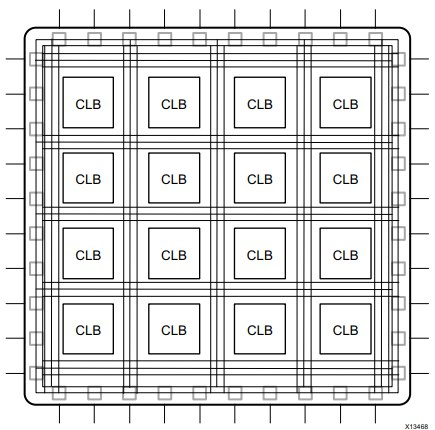
\includegraphics[width=12cm]{figuras/fpga-architecture.jpeg}
		}{
			\Fonte{\cite{fpgaxilinx}.}
		}	
	\end{figure}

Arquiteturas de FPGAs contemporâneas incluem blocos adicionais de \textit{interface}, armazenamento e de processamento específico, tais como blocos MAC, que aumentam a eficiência do dispositivo. Esses elementos adicionais são os seguintes:

\begin{itemize}
    \item Memórias Embarcadas para armazenamento distribuído de dados
    \item \textit{Phase-locked loops (PLLs)} para levar a \textit{FPGA Fabric} em diferentes taxas de clock
    \item Transceptores seriais de alta velocidade
    \item Controladores de memória \textit{Off-chip}
    \item Blocos multiplicadores-acumuladores (\textit{Multiply-accumulate blocks})
    
\end{itemize}

A combinação desses elementos fornece a FPGA a flexibilidade de implementar qualquer algoritmo de software em execução em um processador e representa a arquitetura de uma FPGA contemporânea.


\subsection{A FPGA Virtex Xilinx UltraScale+ VU9P} \label{sec:virtex}
 
 A Xilinx possui famílias de FPGAs, que são fabricadas em nós tecnológicos diversos, sendo as FPGAs \textit{high end} atualmente fabricadas no nó tecnológico de 16nm. A Tabela \ref{Tab:familias} mostra as famílias de acordo com os nós tecnológicos nos quais cada família é fabricada.

 Note que, conforme exemplificado acima com a Xilinx ultrascale+ fabricadas em 16nm, as FPGAs \textit{high end} são fabricadas em nós tecnológicos de dimensões menores, permitindo assim a integração de mais circuitos e unidades lógicas. De uma maneira geral, a FPGA  Virtex Xilinx UltraScale+ VU9P contém 1.182 LUTs, 2.364 flip-flops, 345.9 Mb de memória e 832 de I/O \cite{ultrascale}.

 A informação do custo de uma FPGA como esta não é fácil de se obter, é necessário entrar em contato com a \textit{Xilinx} e atender a pré-requisitos estabelecidos pela empresa para a informação ser oferecida. Porém, em discussões em fóruns e comunidades de desenvolvedores de aplicações para FPGA, estima-se que o custo é de entre $US$ 30,000 e $US$ 50,000. Contudo, é possível acessar aos recursos desta FPGA como um serviço, por meio da computação em nuvem, no ambiente de nuvem Amazon Web Services (AWS). Os conceitos de computação em nuvem e da AWS são discutidos a seguir.

 \begin{table}[!htb]
    \centering
    \caption{Famílias Xilinx de acordo com a tecnologia utilizada}
    \label{Tab:familias}
    \begin{tabular}{cccc}
    \hline 
    \textbf{45 nm}                        & \textbf{28 nm}   & \textbf{20 nm}    & \textbf{16 nm}                                                                                                                                                                                                                                            \\ \hline
    $Spartan & Virtex^{7} & Virtex Ultra Scale & Virtex Ultra Scale^{+}$
    
    \\ \hline
      & $Kintex^{7} & Kintex Ultra Scale & Kintex Ultra Scale^{+}$
     
     \\ \hline
     & $Artix^{7}$  &   &
     \\ \hline
     & $Spartan^{7}$  &   &
     \\ \hline
    \end{tabular}
   
\end{table}


\section{Computação em Nuvem}

Atualmente, os serviços básicos e essenciais como, água, eletricidade, telefone e gás, são entregues de uma forma transparente e são explorados por meio do modelo de pagamento baseado no uso. A mesma ideia tem sido utilizada com os serviços de informática. Neste sentido, plataformas e softwares estão sendo disponibilizados como serviços, por meio de um ambiente de Computação em Nuvem, melhorando a flexibilidade, reduzindo o custo do total do negócio e provendo serviços sob demanda.


A definição de Computação em Nuvem, ou \textit{Cloud Computing}, fornecida pelo National Institute of Standards and
Technology (NIST) diz que a Computação em Nuvem é um modelo para permitir acesso de rede conveniente e sob demanda a um conjunto compartilhado de recursos de computação configuráveis por exemplo, redes, servidores, aplicações de armazenamento  e serviços que podem ser rapidamente provisionados e liberados com esforço mínimo de gerenciamento ou interação com o provedor de serviços \cite{6203873}. Basicamente, a computação em nuvem move a computação e os dados para longe dos desktop e PCs portáteis convencionais para um grande \textit{data center}. Seu principal objetivo é fazer um melhor uso dos recursos distribuídos, combinando-os a fim de alcançar um maior rendimento, além de ser capaz de resolver a computação em grande escala.


A computação em nuvem apresenta cinco principais características, que são as seguintes:
\begin{itemize}
    \item \textit{Self-service} sob demanda: A capacidade dos consumidores em obter, configurar e implementar serviços na nuvem sem a necessidade de intervenção humana por parte do prestador de serviço.
    
    \item Amplo acesso: Diz respeito à disponibilidade dos recursos por meio de uma rede de computadores permitindo que diferentes dispositivos (computadores, tablets, smartphones, etc) possam acessae estes recursos através de mecanismos padronizados.   
    
    \item \textit{Pooling} de recursos: Os recursos de computação (armazenamento, processamento, memória, etc) do provedor de nuvem são agrupados para atender a diversos consumidores usando um modelo \textit{multi-tenant} (multi-inquilino), com diferentes recursos físicos e virtuais atribuídos e reatribuídos dinamicamente, de acordo com a demanda do consumidor.
    
    \item Elasticidade rápida: É a ideia dos recursos computacionais poderem ser rapidamente provisionados ou restringidos de acordo com a necessidade do consumidor.
    
    \item Serviço medido: A quantidade de recursos na nuvem usados pelo consumidor deve ser monitorada, controlada e reportada fornecendo transparência para o fornecedor e o consumidor do serviço utilizado.  Além disso, a partir dessa informação, devem ser estabelecidos os modelos de pagamento.

\end{itemize}


A crescente adoção da utilização de recursos provisionados pela nuvem por parte de pequenas e grandes empresas, se deve aos diversos benefícios que a computação em nuvem tem oferecido, como fácil gerenciamento, início rápido, escalabilidade, transparência de custos, baixo custo de manutenção, potencial para maior segurança, potencial para maior confiabilidade, etc. \cite{5942089}

Atualmente, empresas como a Amazon Web Services, Microsoft Azure, Google Cloud Platform e IBM Cloud fazem parte do grupo dos principais provedores de Computação em Nuvem. Na próxima seção serão discutidos os principais conceitos da Amazon Web Services, por se tratar do provedor que oferece o serviço estudado neste trabalho.  

\subsection{Amazon Web Services (AWS)}

A Amazon Web Services (AWS) é uma plataforma de computação formada por uma coleção de serviços de infra-estrutura, como poder de processamento, opções de armazenamento, redeQuando executa uma instância, o tipo de instância que você especifica determina o hardware do computador host usado para sua instância. Cada tipo de instância oferece uma memória de computação diferente e os recursos de armazenamento são agrupados em famílias de instâncias de acordo com esses recursos e banco de dados que são entregues como um utilitário: sob demanda, disponíveis em segundos, com preços pré-pagos \cite{awsOverview}.

Esses serviços operam a partir de 16 regiões geográficas pelo mundo, os mais centrais e conhecidos desses serviços são Amazon Simple Storage Service (S3), Amazon Elastic Compute Cloud (EC2) e Amazon Relational Database Service (RDS), estes dois primeiros foram utilizados neste estudo, e por isso, serão descritos a seguir.

\begin{itemize}

    \item \textbf{Amazon Simple Storage Service (S3)}: É um serviço de armazenamento de objetos criado para armazenar e recuperar qualquer quantidade de dados de qualquer local: sites e aplicativos móveis, aplicativos corporativos e dados de sensores ou dispositivos da IoT \cite{awsOverview}. Os objetos são organizados em \textit{buckets}, os são quais identificados por uma URI e acessados por meio de um serviço web.
    
    \item \textbf{Amazon Elastic Compute Cloud (EC2)}: Fornece acesso a instâncias (servidores) com recursos computacionais como um serviço sob demanda. O EC2 é uma parte essencial da AWS, pois fornece capacidade de computação escalável para as organizações. Estes são alguns dos recursos forneciso pelo EC2:
    \begin{itemize}
    \item Ambientes de computação virtual, conhecidos como instâncias.
    \item Os modelos pré-configurados para  instâncias, conhecidos como Imagens de máquina da Amazon (AMIs), que empacotam os bits necessários para o servidor (incluindo o sistema operacional e software adicional).
    \item Várias configurações de capacidade de CPU, memória, armazenamento e redes para as instâncias, conhecidas como tipos de instância.
    \item Informações seguras de login para as instâncias usando pares de chave (a AWS armazena a chave pública e o consumidor armazena a chave privada em um lugar seguro).
    \item Volumes de armazenamento para dados temporários que são excluídos quando uma instância é interrompida ou encerrada, conhecidos como volumes de armazenamento de instâncias.
    \item Volumes de armazenamento persistentes para os dados usando o Amazon Elastic Block Store (Amazon EBS), conhecidos como volumes do Amazon EBS.
\end{itemize}
 

Quando uma instância é executada, o tipo de instância especificada determina o hardware do computador host usado para a instância. Cada tipo de instância oferece uma memória de computação diferente e os recursos de armazenamento são agrupados em famílias de instâncias de acordo com esses recursos \cite{awsInstances}. O Amazon EC2 fornece os tipos de instâncias listados na Tabela \ref{Tab:Instancias}.

 
\begin{table}[H]
    \centering
    \caption{Tipos de instâncias do Amazon EC2}
    \label{Tab:Instancias}
    \begin{tabular}{ll}
    \hline 
    \textbf{Família de instâncias}                        & \textbf{Tipos de instância}                                                                                                                                                                                                                                                                                         \\ \hline
    \multicolumn{1}{|l|}{Propósito geral}                 & \multicolumn{1}{l|}{\begin{tabular}[c]{@{}l@{}}t2.nano | t2.micro | t2.small | t2.medium\\  | t2.large | t2.xlarge | t2.2xlarge | m4.large |\\  m4.xlarge | m4.2xlarge | m4.4xlarge | \\ m4.10xlarge | m4.16xlarge | m5.large |\\  m5.xlarge | m5.2xlarge | m5.4xlarge |\\  m5.12xlarge | m5.24xlarge\end{tabular}} \\ \hline
    \multicolumn{1}{|l|}{Otimizadas para computação}      & \multicolumn{1}{l|}{\begin{tabular}[c]{@{}l@{}}c4.large | c4.xlarge | c4.2xlarge | \\ c4.4xlarge | c4.8xlarge | c5.large | \\ c5.xlarge | c5.2xlarge | c5.4xlarge | \\ c5.9xlarge | c5.18xlarge\end{tabular}}                                                                                                       \\ \hline
    \multicolumn{1}{|l|}{Otimizado para memória}          & \multicolumn{1}{l|}{\begin{tabular}[c]{@{}l@{}}r4.large | r4.xlarge | r4.2xlarge | r4.4xlarge | \\ r4.8xlarge | r4.16xlarge | x1.16xlarge | \\ x1.32xlarge | x1e.xlarge | x1e.2xlarge | \\ x1e.4xlarge | x1e.8xlarge |x1e.16xlarge |\\  x1e.32xlarge\end{tabular}}                                                  \\ \hline
    \multicolumn{1}{|l|}{Otimizada para armazenamento}    & \multicolumn{1}{l|}{\begin{tabular}[c]{@{}l@{}}d2.xlarge | d2.2xlarge | d2.4xlarge | \\ d2.8xlarge | h1.2xlarge | h1.4xlarge | \\ h1.8xlarge | h1.16xlarge | i3.large | i3.xlarge | \\ i3.2xlarge | i3.4xlarge | i3.8xlarge | i3.16xlarge\end{tabular}}                                                             \\ \hline
    \multicolumn{1}{|l|}{Computação baseada em GPU, FPGA} & \multicolumn{1}{l|}{\begin{tabular}[c]{@{}l@{}}f1.2xlarge | f1.16xlarge | g3.4xlarge | \\ g3.8xlarge | g3.16xlarge | p2.xlarge | \\ p2.8xlarge | p2.16xlarge | p3.2xlarge | \\ p3.8xlarge | p3.16xlarge\end{tabular}}                                                                                               \\ \hline
    \end{tabular}
   
\end{table}



\end{itemize}

\section{O Serviço Amazon EC2 F1  de Processamento remoto  em   FPGAs na nuvem}\label{sec:servicos amazon}

    Com a grande quantidade de tecnologias e plataformas que estão sendo apresentadas no mercado, os centros de dados dessas aplicações cada vez mais precisam enfrentar o desafio de acelerar cargas de trabalho com tipos de dados complexos, que exigem um poder de processamento que ultrapassa a capacidade de CPUs tradicionais.
    
    As GPUs são amplamente usadas para o processamento de aplicações de análise de dados e de aprendizagem de máquinas. As FPGAs tem sido vistas como uma melhor solução, proporcionando maior desempenho por watt em vários cenários \cite{8119247}, em particular naqueles que fazem uso de aritmética de ponto fixo e não realizam operações de ponto flutuantes. No entanto, a adoção de FPGAs para aceleração de aplicações ainda é limitada devido a dificuldade de implementação tanto de um acelerador eficiente baseado em FPGA,  quanto da infra-estrutura que realiza a comunicação entre o acelerador e a aplicação que fornece e/ou recebe dados da FPGA. 
    
    A fim de facilitar essa comunicação e oferecer um ambiente pronto para o desenvolvimento de acelerações baseadas em FPGAs, a AWS lançou no ano de 2016 as instâncias de computação em nuvem Elastic Compute Cloud (EC2) F1, que são equipadas com FPGAs Xilinx. Essas instâncias permitem uma maior rapidez no desenvolvimento das aplicações por disponibilizarem todos os itens necessários para desenvolver, simular, depurar e compilar código de aceleração de hardware \cite{aws2016f1}.
    
    
    
    Abaixo serão descritos todos os conceitos necessários para o desenvolvimento e implementação de acelerações baseadas em FPGAs, fornecidas pelo AWS EC2 F1.
    
    

  
\subsection{Arquitetura da instância F1} \label{sec:arq}
    
    A implantação do design da aplicação para a FPGA é feita nas instâncias EC2 F1, que são oferecidas em dois tamanhos diferentes e disponibilizam FPGAs Xilinx UltraScale+ VU9P fabricadas em tecnologia de 16 nm. É possível iniciar múltiplas instâncias com 1 ou 8 FPGAs conectadas. Cada placa inclui 64 GiB de memória protegida DDR4 ECC com uma conexão PCIe x16 dedicada.  Cada FPGA contém aproximadamente 2,5 milhões de elementos de lógica e 6.800 mecanismos de processamento de sinais digitais (DSP) \cite{aws2016f1}. % verificar essa citação do site
    
    As especificações mais detalhadas de cada tipo de instâncias F1 são mostradas na Tabela \ref{Tab:F1}. 
        
    \begin{table}[!htb]\tiny
    \centering
     \caption{Detalhes da Instância F1}
    \label{Tab:F1}
    \begin{tabular}{lccccccc}
    \hline
    \multicolumn{1}{l}{Tipo de Instância}&\multicolumn{1}{l}{FPGAs }&\multicolumn{1}{l}{DDR-4(Gib)}&\multicolumn{1}{l}{vCPUs}&\multicolumn{1}{l}{Memória (GiB)}&\multicolumn{1}{l}{Arm. NVMe (GB)}&\multicolumn{1}{l}{Largura de Banda} \\ \midrule 
    
    f1.2xlarge & 1 & 4 x 16 & 8 & 122 & 1 x 470 & Até 10 Gbps\\   \midrule
    f1.16xlarge & 8 & 32 x 16 & 64 & 976 & 4 x 940 & 25  Gbps\\   \midrule

    \end{tabular}
    \end{table}
    


A aceleração baseada em FPGA na AWS é uma estratégia de coprocessamento, a FPGA é ligada aos pós-processadores via PCI Express (PCIe), essa conexão PCIe também permite a comunicação entre as FPGAs da instância f1.16xlarge. Assim, uma típica aplicação para a instância f1 inclui um software executando nos processadores host comunicando dados e instruções, através de uma interface PCIe, para a FPGA, que contém a aplicação que foi desenvolvida e carregada na FPGA. A Figura \ref{fig:f1-architecture} detalha esse processo de comunicação.


   
\begin{figure}[h!] 
   	    \captionsetup{width=12cm}%Da mesma largura que a figura
		\Caption{\label{fig:f1-architecture} Como uma aceleração de FPGA funciona na AWS}
		\UFCfig{}{
			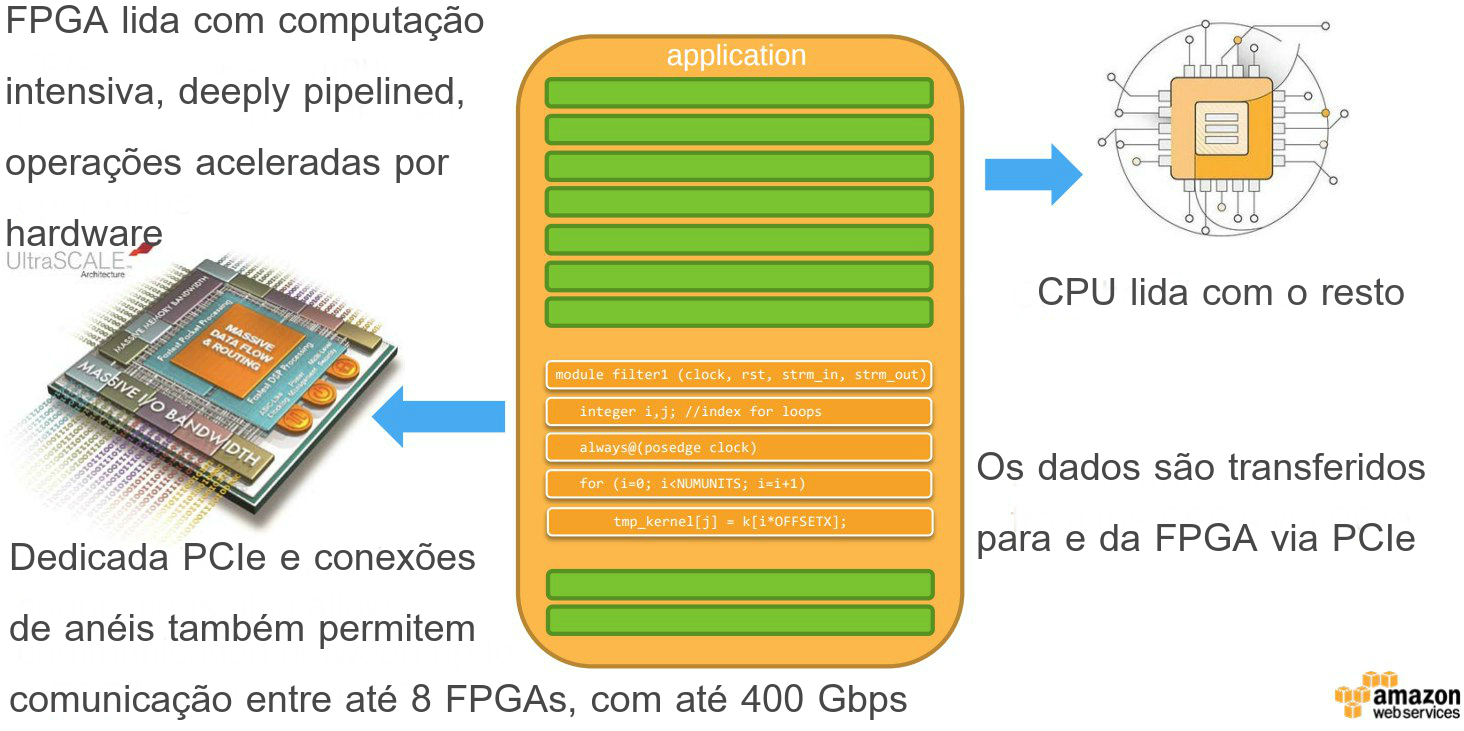
\includegraphics[width=12cm]{figuras/f1-architecture.jpg}
		}{
			\Fonte{\cite{aws2016f1}.}
		}	
	\end{figure}
    

\subsection{Desenvolvimento de Cores} \label{sec:dev}

Para desenvolver as aplicações FPGAs é necessário seguir um fluxo de programação proposto pela AWS. Esse fluxo é descrito pelos seguintes passos:

\begin{enumerate}
    \item Desenvolver a \textbf{Lógica Customizada (\textit{Custom Logic - CL)}} para a FPGA utilizando as ferramentas de desenvolvimento da Xilinx, disponíveis na \textbf{\textit{FPGA Deveploper AMI}}, combinadas com o \textbf{Kit de desenvolvimento - HDK }.
    
    \item Combinar a CL com uma lógica fornecida pela AWS chamada de \textbf{FPGA \textit{Shell}}.
    
    \item Criar uma \textbf{\textit{Amazon FPGA Image (AFI)}} a partir da CL construída.
    
    \item Carregar a AFI gerada em uma FPGA conectada à instância F1 ou disponilizar no AWS Marketplace.
\end{enumerate}

Os recursos ofertados pela AWS citados na descrição do fluxo de desenvolvimento serão discutidos nas próximas seções.

\subsubsection{ FPGA Developer AMI} \label{sec:ami}

Para permitir um desenvolvimento rápido de acelerações de hardware, a AWS disponibiliza uma AMI para desenvolvedores de FPGA, a \textit{FPGA Developer AMI}, que é um ambiente de desenvolvimento pré-definido, com scripts e ferramentas para o desenvolvimento, compilação e simulação do design FPGA, pronto para ser executado em uma instância EC2. Por se tratar de uma ambiente de desenvolvimento, \textit{FPGA Developer AMI} normalmente não é executada em uma instância F1, mas em outros tipos de instâncias EC2, em uma instância que não contém uma FPGA. A AMI pode ser implantada em uma variedade de tipos e tamanhos de instâncias EC2, como por exemplo a M4 que é para propósitos gerais, a R4 que é otimizada para memória, a C4 que é otimizada para computação, ou a T2, que tem um baixo custo. esta última deve ser usada apenas para o design e simulação, não sendo indicada para a síntese ou PAR (\textit{place-and-route}).

\textit{FPGA Developer AMI} está disponível no AWS Marketplace, onde não são aplicados custos para o uso da AMI e suas ferramentas, apenas são cobrados os custos por hora de execução da instância EC2 escolhida.


\subsubsection{Kit de desenvolvimento - HDK e SDK} \label{sec:hdk}
    
    A AWS disponibiliza o repositório AWS-FPGA na plataforma github, no endereço https://github.com/aws/aws-fpga, que contém os kits de desenvolvimento de hardware e software. Esses kits incluem duas partes: o HDK e o SDK.
    
    O HDK é um diretório onde estão disponíveis todos os arquivos de design e scripts necessários para criar uma \textit{Amazon FPGA Image (AFI)} a partir de um projeto RTL(Verilog/VHDL), que é uma imagem que contém o bitstream pronto para ser implementado em uma FPGA. Para usá-lo, o desenvolvedor deve baixar o HDK instalá-lo em seu ambiente de desenvolvimento, na nuvem ou local.
    
    Nesse diretório estão inclusos todos os scripts de criação do ambiente de desenvolvimento, simulação, compilação e criação da AFI. A instalação do HDK pode ser feita em qualquer servidor local ou em uma instância EC2. O uso do HDK é necessário apenas se for preciso criar uma AFI e não utilizar uma AFI pré-construída.
    
    O diretório SDK inclui todos os drives e o ambiente de execução exigidos em qualquer instância EC2 FPGA. Esses drives e ferramentas são usados para a interação com as AFI pré-construídas que serão carregadas nas FPGAs disponíveis nas instâncias EC2 F1.
    
    Além disso, o SDK contém as ferramentas de gerenciamento da \textit{Amazon FPGA Image (AFI)}, que inclui tanto o código fonte para as ferramentas de gerenciamento da AFI, quanto as descrições detalhadas dos comandos a serem usados  uma instância F1.
    

     
\subsubsection{Lógica Customizada (Custom Logic - CL)} \label{sec:cl}

A Lógica Customizada, ou \textit{Custom Logic - CL}, é o design completo desenvolvido para a FPGA. A combinação da CL com a AWS Shell tem como resultado um \textit{Design Checkpoint (DCP)} e não um bitstream, esse é gerado pela AWS depois que o desenvolvedor envia o DCP \cite{awsfaq}. 

Existe uma interface entre a CL e uma aplicação real em execução no espaço do usuário do linux durante o tempo de execução. Nessa interface há duas partes: \textit{Management} e \textit{Runtime}. A Figura \ref{fig:cl} mostra uma visão de alto nível desses componentes e como eles se relacionam com a FPGA.

\begin{figure}[htb!] 
   	    \captionsetup{width=15cm}%Da mesma largura que a figura
		\Caption{\label{fig:cl} Visão do programador da Custom Logic}
		\UFCfig{}{
			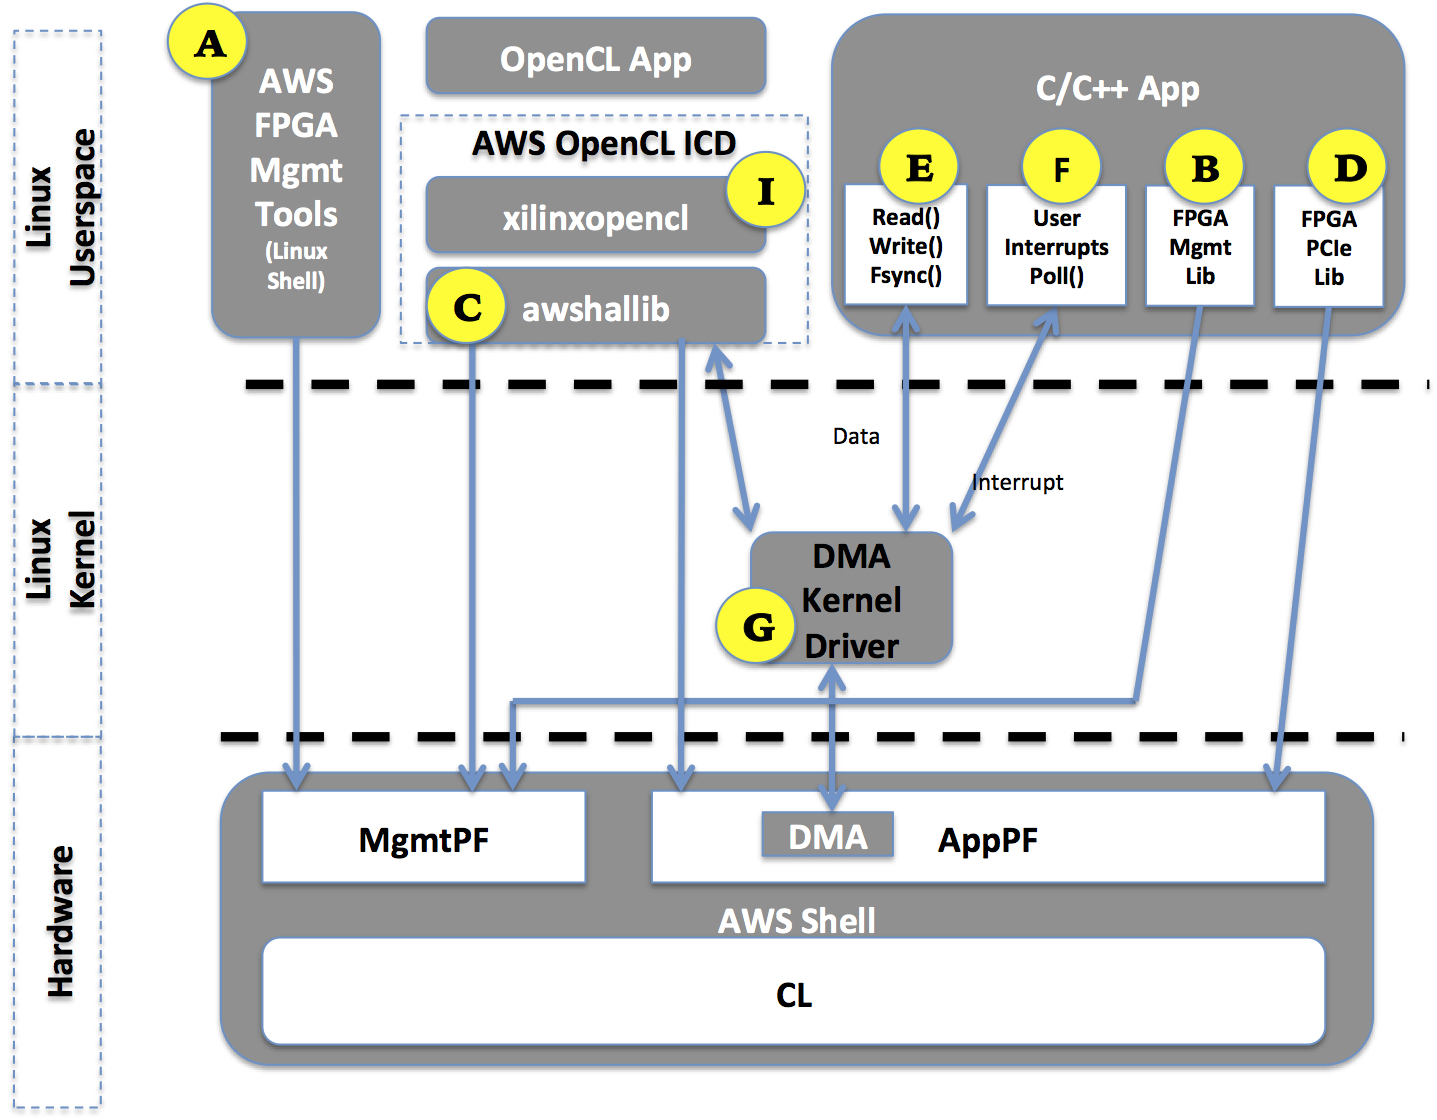
\includegraphics[width=16cm]{figuras/cl.png}
		}{
			\Fonte{\cite{awscl}.}
	}		
\end{figure}

\begin{enumerate}
    \item \textbf{Management Interface}: necessário para carregar/limpar uma AFI, verificar o status de uma AFI, depurar a AFI, os LEDs Emulados e os  DIP Switches Emulados \cite{awscl}. A interface de gerenciamento é fornecida em uma das três opções, uma ou mais podem ser usadas simultaneamente:
    
   \textbf{[A]} Como comandos shell do linux chamados de  FPGA Management Tools. 
    
    \textbf{[B]} Como uma biblioteca C chamada de FPGA Management Lib para ser compilada com a aplicação C/C++ do desenvolvedor.
    
    \textbf{[C]} Pré-integrado com OpenCL runtime library.
    
    \item \textbf{Runtime Code}: necessário para leitura/gravação de/para a lógica personalizada, tratamento de interrupções e uso do DMA \cite{awscl}. Isso é fornecido por:
    
    \textbf{[D]} FPGA PCIe Lib é uma biblioteca C usada para acessar o espaço de memória da FPGA atrás do AppPF PCIe BARs (definidos no FPGA Shell), do espaço de aplicação Linux, como leitura/gravação, para registrar espaço ou transmitir mensagens. Esta biblioteca pode ser compilada e vinculada na aplicação C/C++ do desenvolvedor.
    
    \textbf{[E]} Uma  Interface DMA usando padrão  POSIX API como open()/read()/write() para ser usada em qualquer aplicação C/C++ para transferência de dados usando DMA. Essa interface de DMA requer a instalação do driver de kernel  AWS EDMA - marcado como item \textbf{[G]}.
    
    \textbf{[F]} Um Espaço de usuário de notificação interrupção/evento usando padrão  POSIX API like open() and poll(), para ser usado em qualquer aplicação C/C++. Essa interface interrupção/evento requer a instalação do driver de kernel  AWS EDMA - marcado como item \textbf{[G]}.
    
    \textbf{[I]} Uma biblioteca OpenCL ICD que se vincula a aplicação de tempo de execução openCL, como o gerado pelo SDAccel da Xilinx.
    

\end{enumerate}



\subsubsection{FPGA Shell} \label{sec:shell}

O \textit{AWS Shell} é a parte da FPGA que é fornecida e gerenciada pela AWS. É uma Lógica responsável por cuidar dos periféricos externos FPGA, PCIe, DRAM e Interrupções.Ele  implementa as tarefas não diferenciadas de desenvolvimento e de trabalho pesado, como configurar a interface PCIe, download de AWS FPGA Image, segurança, monitoramento de integridade, métricas e ganchos de depuração \cite{awsfaq}. Cada FPGA implantada na nuvem inclui um AWS Shell e as interfaces da \textit{custom logic} do desenvolvedor com as interfaces disponíveis do AWS Shell.

A Tabela \ref{Tab:shell} e a Figura \ref{fig:shell}  resumem as várias interfaces entre o Shell e o CL.



\begin{figure}[H] 
   	    \captionsetup{width=15cm}%Da mesma largura que a figura
		\Caption{\label{fig:shell} Interfaces Shell}
		\UFCfig{}{
			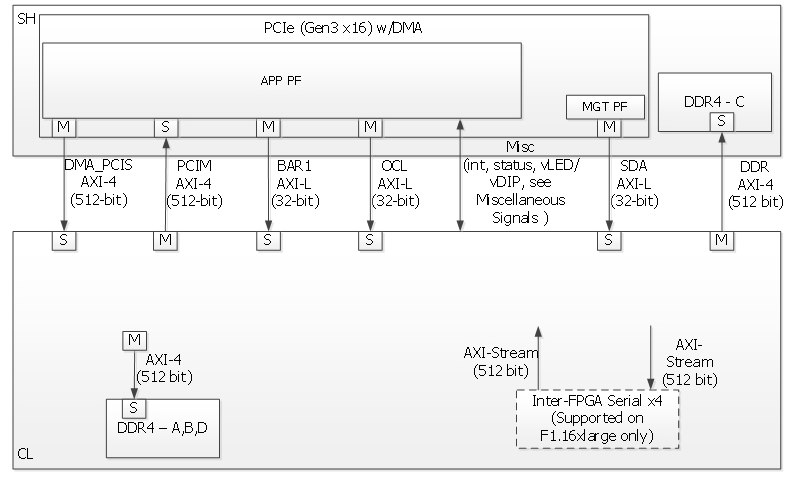
\includegraphics[width=16cm]{figuras/shell.jpeg}
		}{
			\Fonte{\cite{awsshell}.}
	}		
\end{figure}


      
\begin{table}[H]
    \centering
     \caption{Interfaces Shell}
    \label{Tab:shell}
     \begin{tabular}{|l|l|}
    \hline
    \textbf{Interface} & \textbf{Descrição}                                                                                                                    \\ \hline
    Clocks e Resets    & Existem vários clocks e resets fornecidos pelo Shell para o CL                                                                        \\ \hline
    DDR4               & \begin{tabular}[c]{@{}l@{}}A interface principal para os controladores DDR4 utiliza uma\\  interface AXI-4\end{tabular}               \\ \hline
    DMA\_PCIS          & \begin{tabular}[c]{@{}l@{}}A interface PCIe Slave (PCIS) é uma interface AXI-4 usada \\ para transações PCIe de entrada\end{tabular}  \\ \hline
    PCIM               & \begin{tabular}[c]{@{}l@{}}A interface PCIe Master (PCIM) é uma interface AXI-4 usada \\ para transações PCIe de saída\end{tabular}   \\ \hline
    SDA                & \begin{tabular}[c]{@{}l@{}}A interface SDA é uma interface AXI-Lite associada ao MgmtPF\\  e ao BAR4\end{tabular}                     \\ \hline
    OCL                & \begin{tabular}[c]{@{}l@{}}A interface OCL é uma interface AXI-Lite associada ao AppPF e \\ ao BAR0\end{tabular}                      \\ \hline
    BAR1               & \begin{tabular}[c]{@{}l@{}}The BAR1 Interface is an AXI-Lite interface associated with AppPF\\  and BAR1\end{tabular}                 \\ \hline
    Interrupts         & Existem 16 interrupções de usuário disponíveis                                                                                        \\ \hline
    Miscellaneous      & \begin{tabular}[c]{@{}l@{}}Existem vários sinais genéricos, como ID's, status, contadores, etc.,\\ entre o Shell  e o CL\end{tabular} \\ \hline
    \end{tabular}
\end{table}

A plataforma FPGA da F1 inclui as seguintes interfaces externas:

\begin{itemize}
    \item Um x16 PCI Express 3.0 Interface.
    \item 
Quatro interfaces DDR4 RDIMM, cada interface é de 72 bits, incluindo ECC.
\end{itemize}
 
Em relação a representação PCIe FPGA para instância do EC2, Existem duas funções físicas PCIe (Physical Functions - PFs) apresentadas à instância F1:

\begin{itemize}
    \item Management PF - Essa PF é usada para o gerenciamento da FPGA e as bibliotecas de gerenciamento FPGA. a Management PF fornece acesso a várias funções de controle, como Virtual-LED, Virtual-DIPSwitch, JTAG virtual, métricas de FPGA e gerenciamento de AFI (carga, limpeza, etc ...) \cite{awsshell}.
    
    \item Application PF (AppPF) - A AppPF é usado para funcionalidades específica do CL.
\end{itemize}

\paragraph{Amazon FPGA Image (AFI)} \label{sec:afi}
 
 Uma \textit{Amazon FPGA Image} é o código FPGA compilado que é carregado em um FPGA na AWS para executar a CL criada pelo desenvolvedor. As AFIs são mantidas pela AWS de acordo e associados à conta da AWS que os criou. O AFI inclui o CL e o \textit{AWS FPGA Shell} \cite{awsfaq}.
 
 Após a conclusão do design, é possível registrar uma Amazon FPGA Image (AFI), que é uma imagem de FPGA que será carregada na FPGA conectada à instância e poderá ser reusada muitas vezes e em quantas instâncias F1 for desejadas.  

Após o processo da criação de uma AFI são fornecidos as seguintes identificadores referentes a AFI criada :
\begin{itemize}

\item FPGA Image Identifier ou AFI ID: este é o ID principal, usado para gerenciar a AFI através dos comandos AWS EC2 CLI e AWS SDK APIs. Este ID é regional, ou seja, se uma AFI é copiado em várias regiões, ele terá uma  AFI ID única diferente em cada região. Um exemplo de AFI ID é afi-06d0ffc989feeea2a. 

\item Global FPGA Image Identifier ou AGFI ID: esta é uma identificação global que é usada para se referir a uma AFI dentro de uma instância F1. Por exemplo, para carregar ou limpar um AFI de um slot FPGA, você usa o AGFI ID. Uma vez que as  AGFI  IDs são globais (por design), permite copiar uma combinação de AFI / AMI para várias regiões, e elas funcionarão sem requerer nenhuma configuração adicional. Um exemplo AGFI ID é agfi-0f0e045f919413242.

\end{itemize}


\subsection{Tarifação} \label{sec:tarifacao}

Os custos gerados ao desenvolver um aplicação para FPGA na AWS dizem respeito a quantidade de horas que as instâncias, usadas para o desenvolvimento e a instância F1, são executadas. Cada instância tem um custo por hora. As instâncias F1 apresentam os seguintes custos:

\begin{itemize}
    \item f1.2xlarge: USD\$1.65 por hora.
    
    \item f1.16xlarge: USD\$13.2 por hora.
\end{itemize}


    




	\chapter{Revisão de Aplicações da EC2 F1}
\label{cap:revisao-de-aplicacoes}
	\chapter{Metodologia de Desenvolvimento}
\label{chap:metodologia}

Neste capítulo será detalhado o trabalho proposto por essa monografia, um estudo sobre a utilização das instâncias EC2 F1 como recurso didático para a disciplina de Sistemas Eletrônicos Digitais Reconfiguráveis (SEDR). Serão apresentadas a metodologia utilizada, todas as práticas realizadas e as ferramentas utilizadas.

\section{Metodologia Utilizada}\label{sec: metodologia-utilizada}

As metodologia adotada para a execução deste trabalho pode ser descrita pelas etapas mostradas na Figura \ref{fig:metodologia}:



\begin{figure}[htb!] 
   	    \captionsetup{width=15cm}%Da mesma largura que a figura
		\Caption{\label{fig:metodologia} Metodologia}
		\UFCfig{}{
			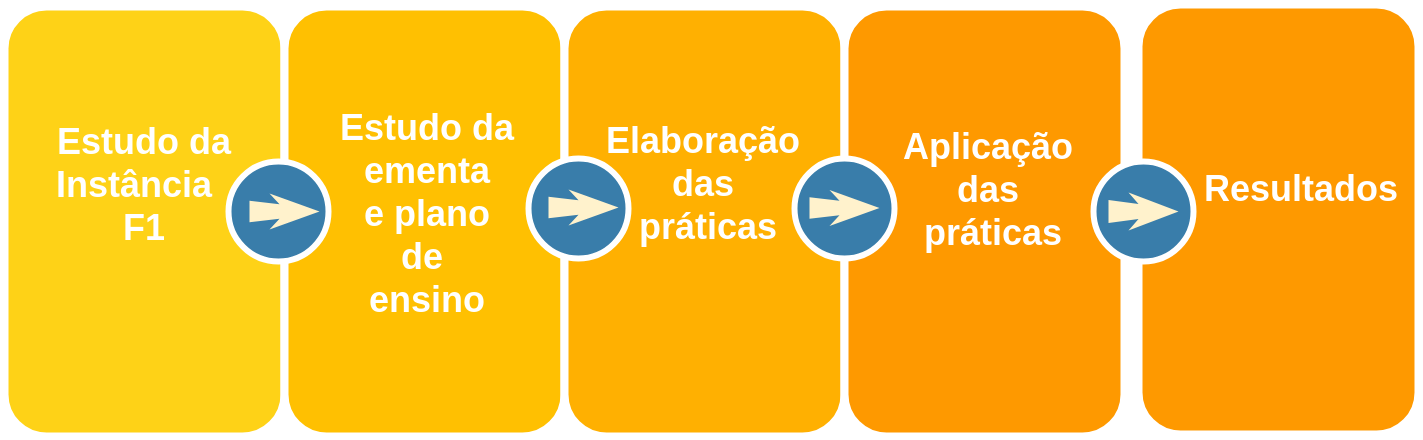
\includegraphics[width=16cm]{figuras/metodologia.png}
		}{
			\Fonte{Próprio Autor.}
	}		
\end{figure}
    
\begin{enumerate}
    \item \textbf{Estudo da Instância F1:} Primeiramente, foi realizado um estudo das instâncias EC2 F1 com o intuito de identificar as possibilidades que esse recurso poderia oferecer para o seu uso no ensino de FPGA.
    
    \item \textbf{Estudo da ementa e plano de ensino da Disciplina de SEDR:} Em seguida, deu-se início ao estudo da ementa e do plano de ensino da disciplina de SEDR para que a utilização das instâncias EC2 F1 fosse adequada da melhor forma possível ao plano de ensino.
    
    \item \textbf{Elaboração das práticas:} Baseando-se nos estudos já realizados e na documentação da Amazon Web Services, as práticas de laboratório foram idealizadas de forma a oferecer um conhecimento geral do processo de desenvolvimento de aplicações para FPGA com o serviço EC2 F1.
    
    \item \textbf{Aplicação das práticas:} Após a elaboração e testes das práticas, iniciou-se a fase de aplicação em laboratório.
    
    \item \textbf{Resultados:} Finalmente, nesta última etapa da metodologia foi analisada a eficácia do uso das instâncias EC2 F1 como recurso didático para a disciplina de SEDR através da aplicação das práticas e de análise de questionários respondidos pelos alunos ao final de cada prática.
	  
\end{enumerate}

  
\section{Contextualização}\label{sec: contextuaizacao}

O trabalho foi realizado no Departamento de Teleinformática da Universidade Federal do Ceará. As práticas foram aplicadas em dois laboratórios deste mesmo departamento para alunos de graduação.

As práticas foram aplicadas na disciplina de SEDR, que é um componente optativo da estrutura curricular do Curso de Graduação em Engenharia de Computação e é ofertada no sétimo semestre da graduação. A mesma possui  uma carga horária de 64 horas (vide ANEXO A - Ementa de SEDR) e tinha o total de 8 alunos matriculados. 

De acordo com a ementa, a carga horária total da disciplina é dividida igualmente entre teoria e prática, ou seja, são utilizadas 32 horas para a teoria e 32 horas para a pŕatica. A carga horária reservada para a  aplicação das práticas desenvolvidas neste trabalho foi de 10 horas, dessa quantidade, 2 horas foram utilizadas para uma aula teórica sobre a Amazon Web Services e o serviço EC2 F1 e as 8 horas restantes foram reservadas para a aplicação das práticas, levando em consideração apenas as atividades desenvolvidas no laboratório durante o horário da aula.

As práticas foram realizadas no Laboratório de Informática (LI) e no Laboratório de Hardware do Departamento de Teleinformática. No primeiro, foram realizadas as práticas 1 e 2 que usam o acesso remoto as instâncias F1. As práticas 3 e 4 foram realizadas no Laboratório de Hardware, pois se utilizou máquinas virtuais, disponíveis nesse laboratório, que continham o kit de desenvolvimento da AWS,o HDK e o SDK, e o ambiente de desenvolvimento da Xilinx SDSoC, que contém o Vivado com uma licença específica para a FPGA Virtex UltraScale+ VU9P, permitindo  o desenvolvimento local (on premises) das pŕaticas.

\section{Ferramentas Utilizadas}\label{sec: ferramentas}

Esta seção detalha as ferramentas que foram utilizadas para a realização das atividades de labotório.

\subsection{Software}\label{sec: software}

\subsubsection{AWS CLI}\label{sec: aws-cli}


\subsubsection{GitHub}\label{sec: github}


\subsubsection{Vivado}\label{sec: vivado}

\subsubsection{VMware}\label{sec: vmware}


\subsection{Hardware}\label{sec: Hardware}

O hardware utilizado foram os computadores dos próprios laboratórios.
	\chapter{Resultados}
\label{chap:resultados}

Texto texto texto texto texto texto texto texto texto texto texto texto texto texto texto texto texto texto texto texto texto texto texto texto texto texto texto texto texto texto texto texto texto texto texto texto texto texto texto texto texto texto texto texto texto texto texto texto texto texto texto texto texto texto texto texto texto texto texto texto texto texto texto texto texto texto texto texto texto.

\section{Resultados do Experimento A}
\label{sec:resultados-do-experimento-a}

Procure deixar as figuras dos resultados o maior possível preenchendo as margens do documento que possui $16~cm$.

\begin{figure}[h!]
        \captionsetup{width=16cm}
		\Caption{\label{fig:tensaoimpedanciahumana} Gráfico de tensão considerando a impedância humana}
		%\centering
		\UFCfig{}{
			\fbox{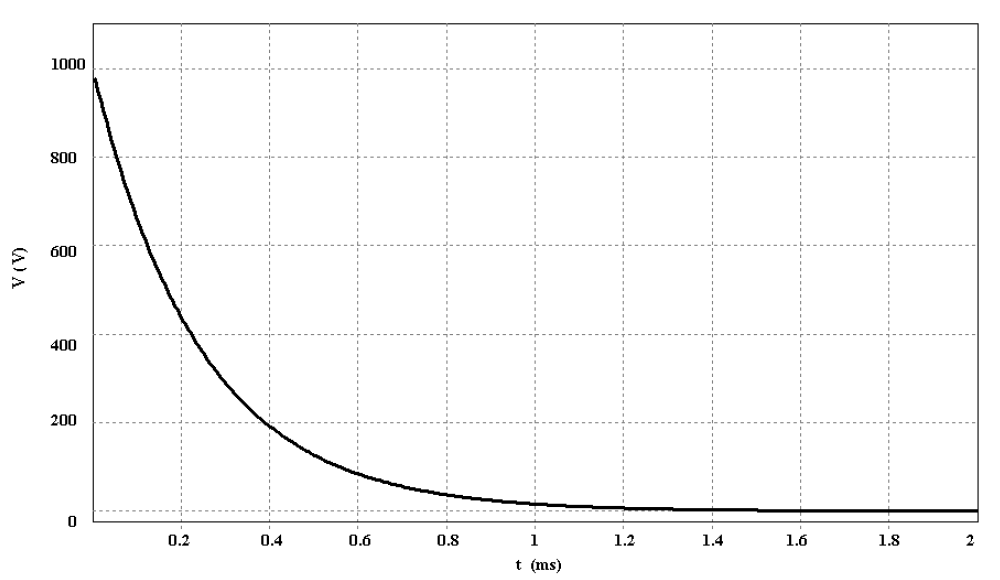
\includegraphics[width=16cm]{figuras/tensaoimpedanciahumana}}
		}{
			\Fonte{o autor.}
		}	
\end{figure}

Texto texto texto texto texto texto texto texto texto texto texto texto texto texto texto texto texto texto texto texto texto texto texto texto texto texto texto texto texto texto texto texto texto texto texto texto texto texto texto texto texto texto texto texto texto texto texto texto texto texto texto texto texto texto texto texto texto texto texto texto texto texto texto texto texto texto texto texto texto.

\begin{figure}[h!]
	\captionsetup{width=16cm}
	\Caption{\label{fig-grafico-1}Produção anual das dissertações de mestrado e teses de doutorado entre os anos de 1990 e 2008}		
	\IBGEtab{}{
		\fbox{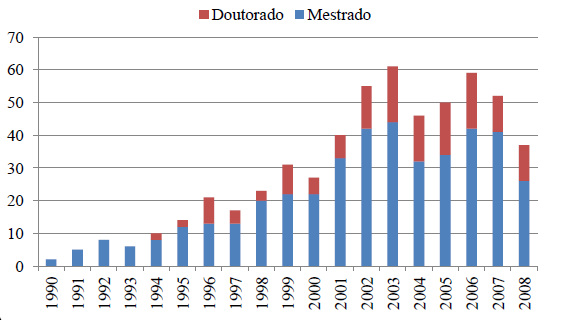
\includegraphics[width=16cm]{figuras/figura-3}}
	}{
	\Fonte{o autor.}
}
\end{figure}

Texto texto texto texto texto texto texto texto texto texto texto texto texto texto texto texto texto texto texto texto texto.

Texto texto texto texto texto texto texto texto texto texto texto texto texto texto texto texto texto texto texto texto texto texto texto texto texto texto texto texto texto texto texto texto texto texto texto texto texto texto texto texto texto texto texto texto texto texto texto texto texto texto texto texto texto texto texto texto texto texto texto texto texto texto texto texto texto texto texto texto texto.

\section{Resultados do Experimento B}
\label{sec:resultados-do-experimento-b}

Texto texto texto texto texto texto texto texto texto texto texto texto texto texto texto texto texto texto texto texto texto texto texto texto texto texto texto texto texto texto texto texto ..

\begin{table}[h!]	
	%\centering
	\captionsetup{width=11.3cm}%ATENÇÃO: Ajuste a largura do título
	\Caption{\label{tab:notas} Notas dos participantes nas avaliações A, B e C}	
	\IBGEtab{}{
		\begin{tabular}{crrr}
			\toprule
			Identificação dos participantes & Avaliação A & Avaliação B &                        Avaliação C \\
			\midrule \midrule
			Participante 1 & 7 & 9 & 10\\
			Participante 2 & 8 & 2 & 1\\
			Participante 3 & 5 & 10 & 6 \\
			Participante 4 & 3 & 1 & 4\\
			Participante 5 & 2 & 4 & 1\\
			Participante 6 & 0 & 7 & 2\\
			\bottomrule
		\end{tabular}
	}{
	\Fonte{o autor.}
}
\end{table}

 Texto texto Referenciando a \autoref{tab:notas}  texto texto texto texto texto texto texto texto texto texto texto texto texto texto texto texto texto texto texto texto texto texto texto texto texto texto texto texto texto texto.Texto texto texto texto texto texto texto texto texto texto texto texto texto texto texto texto texto texto texto texto texto.

Texto texto texto texto texto texto texto texto texto texto texto texto texto texto texto texto texto texto texto texto texto texto texto texto texto texto texto texto texto texto texto texto texto texto texto texto texto texto texto texto texto texto texto texto texto texto texto texto texto texto texto texto texto texto texto texto texto texto texto texto texto texto texto texto texto texto texto texto texto.Texto texto texto texto texto texto texto texto texto texto texto texto texto texto texto texto texto texto texto texto texto texto texto texto texto texto texto texto texto texto texto texto texto texto texto texto texto texto texto texto texto.

Texto texto texto texto texto texto texto texto texto texto texto texto texto texto texto texto texto texto texto texto texto texto texto texto texto texto texto texto texto texto texto texto texto texto texto texto texto texto texto texto texto texto texto texto texto texto texto texto.Texto texto texto texto texto texto texto texto texto texto texto texto texto texto texto texto texto texto texto texto texto.

Texto texto  Referenciando a \autoref{tab:notas}  texto texto texto texto texto texto texto texto texto texto texto texto texto texto texto texto texto texto texto texto texto texto texto texto texto texto texto texto texto texto texto texto texto texto texto texto texto texto texto texto texto texto texto texto texto texto texto texto texto texto texto texto texto texto texto texto texto texto texto texto texto texto texto texto texto texto texto.
	\chapter{Conclusões e Trabalhos Futuros}
\label{chap:conclusoes-e-trabalhos-futuros}

Parte final do texto na qual se apresentam as conclusões apoiadas no desenvolvimento do assunto. É a recapitulação sintética dos resultados obtidos. Pode apresentar recomendações e sugestões para pesquisas futuras.

%\label{sec:contribuicoes-do-trabalho}



%\label{sec:limitacoes}








	
	%Elementos pós-textuais	
	\bibliography{3-pos-textuais/referencias}
%	\imprimirglossario	
	\imprimirapendices
		% Adicione aqui os apendices do seu trabalho
		\apendice{Roteiro das práticas de laboratório}
\label{ap:A}

Os roteiros das práticas também estão disponíveis no GitHub, no link: \url{https://github.com/vanros/Praticas-SEDR-AWS}.


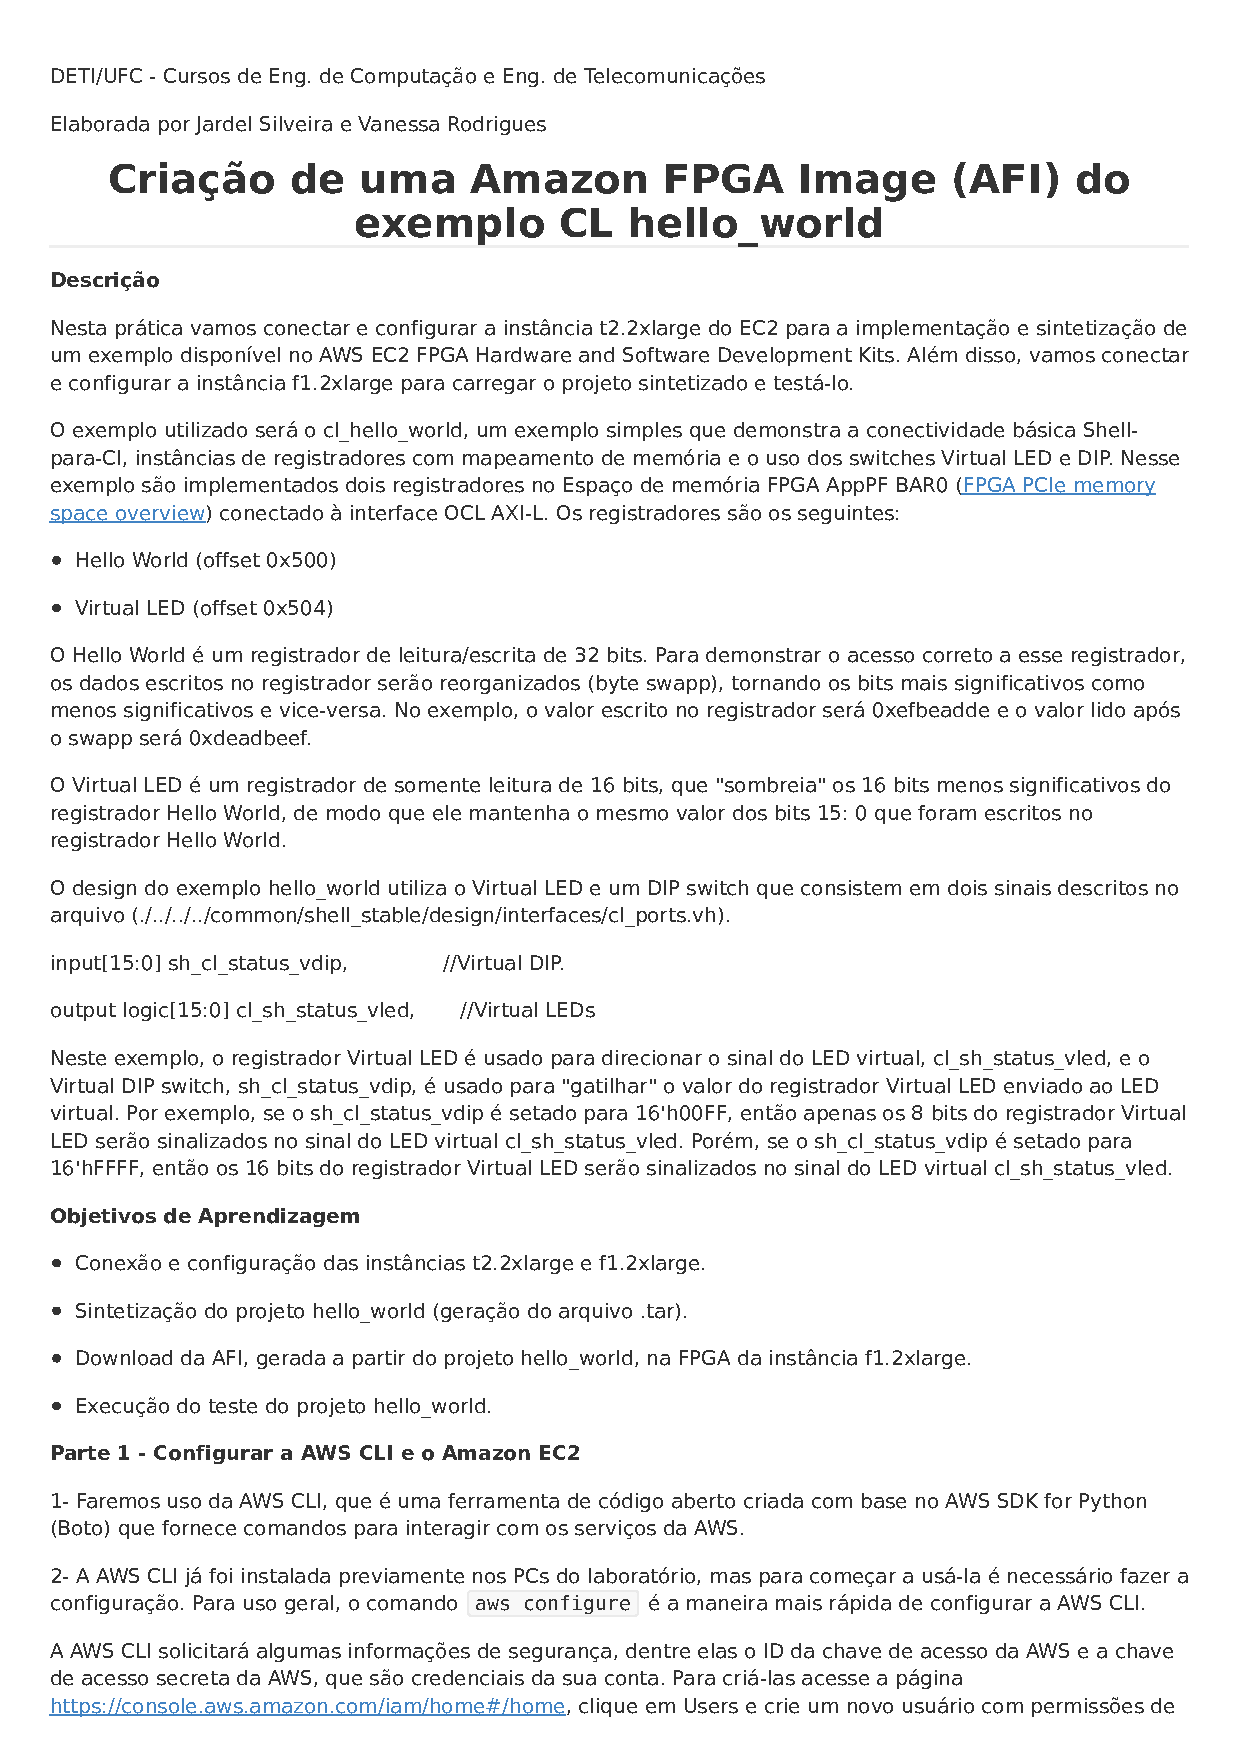
\includepdf[pages={-}]{3-pos-textuais/apendices/Pratica1.pdf}

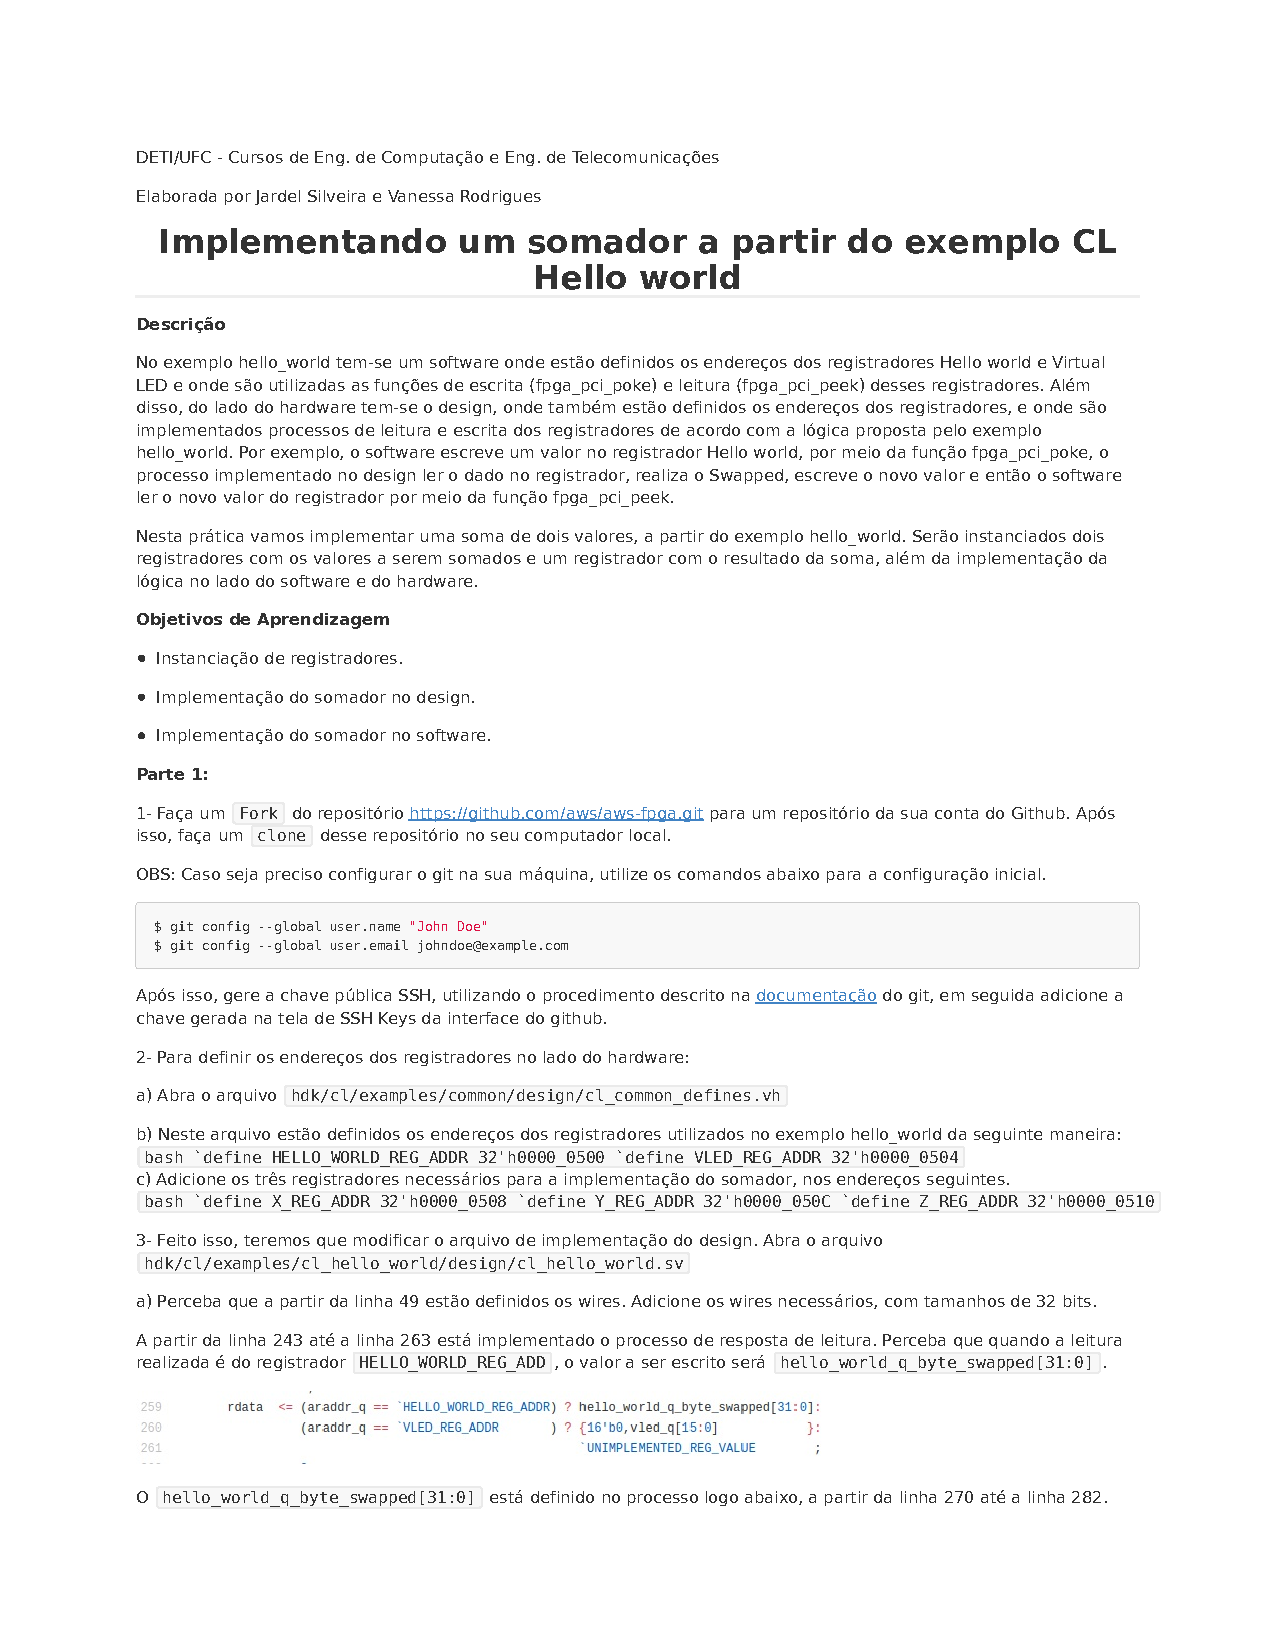
\includepdf[pages={-}]{3-pos-textuais/apendices/Pratica2.pdf}

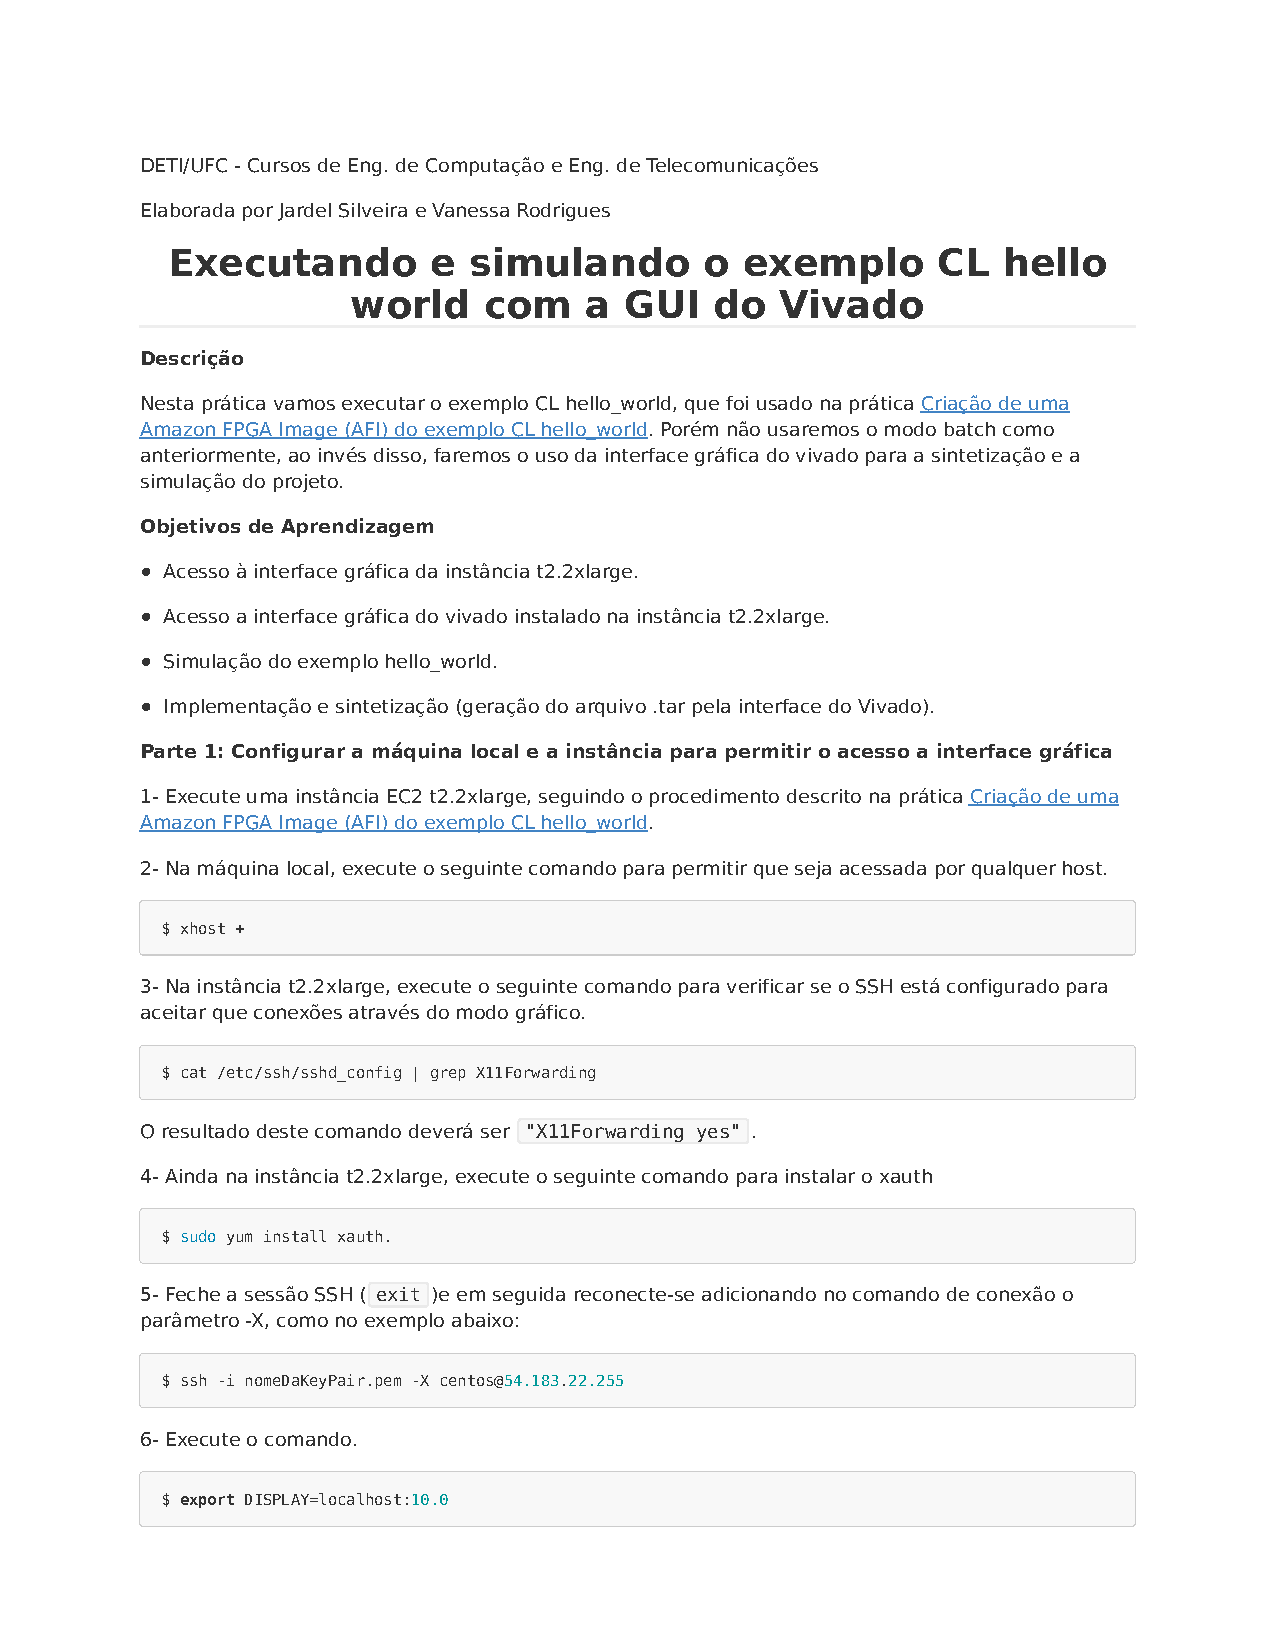
\includepdf[pages={-}]{3-pos-textuais/apendices/Pratica3.pdf}

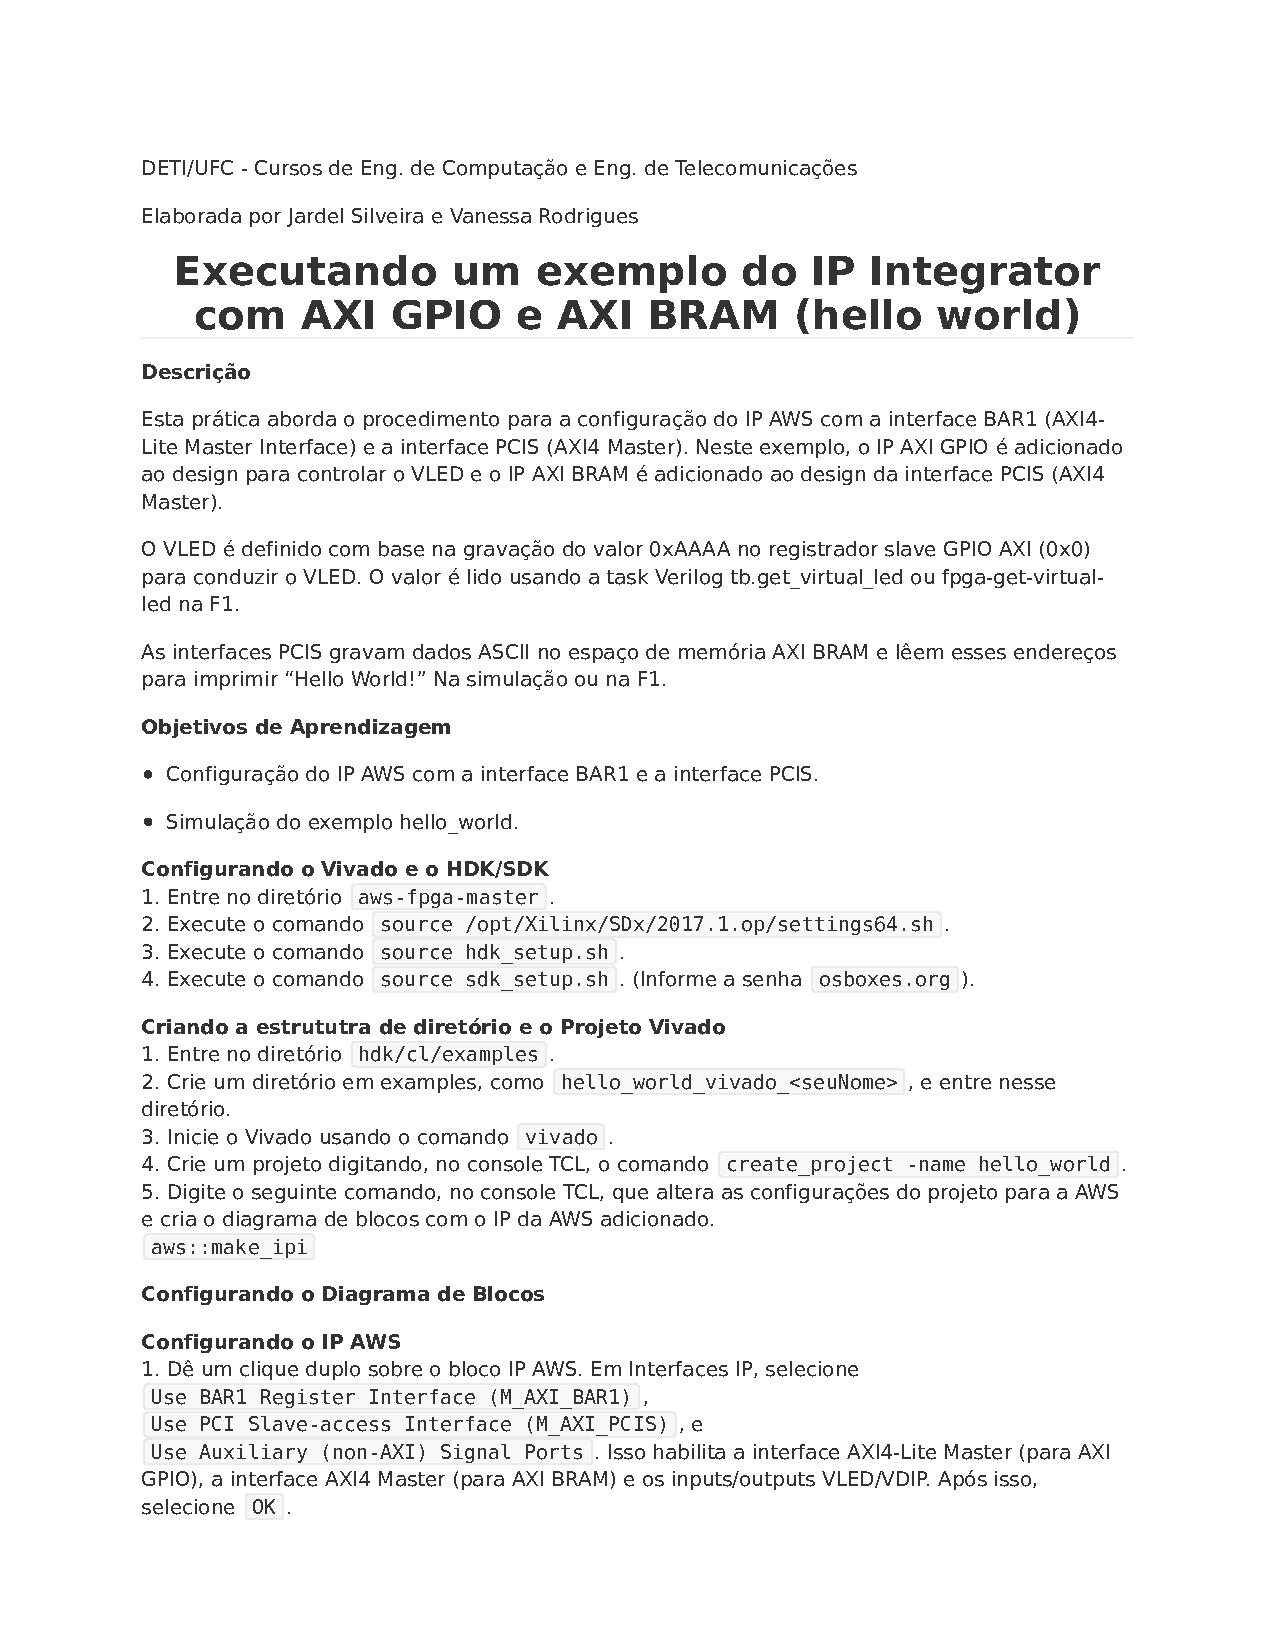
\includepdf[pages={-}]{3-pos-textuais/apendices/Pratica4.pdf}
		\apendice{Questionário utilizado para...}
\label{ap:B}

\begin{questao}
	\item Esta é a primeira questão com alguns itens:
		\begin{enumerate}
			\item Este é o primeiro item
			\item Segundo item
		\end{enumerate}
	\item Esta é a segunda questão:
		\begin{enumerate}
			\item Este é o primeiro item
			\item Segundo item
		\end{enumerate}
	\item Lorem ipsum dolor sit amet, consectetur adipiscing elit. Nunc dictum sed tortor nec viverra. consectetur adipiscing elit. Nunc dictum sed tortor nec viverra.
		\begin{enumerate}
			\item consectetur
			\item adipiscing
			\item Nunc
			\item dictum
		\end{enumerate}
\end{questao}

		\apendice{Códigos-fontes utilizados para...}
\label{ap:C}

\lstinputlisting[language=C++,caption={Hello World em C++}]{figuras/main.cpp}


\begin{lstlisting}[language=Java,caption={Hello World em Java}]
public class HelloWorld {
	public static void main(String[] args) {
		System.out.println("Hello World!");
	}
}
\end{lstlisting}


		\apendice{\textit{IEEE CEFC 2016}}
\label{ap:D}

\textit{Digest} submetido ao \textit{The 17th Biennial Conference on Eletromagnetic Field Computation, Miami FL - NOV 13-16, 2016, USA}.

%Código fonte para inserir um arquivo em PDF
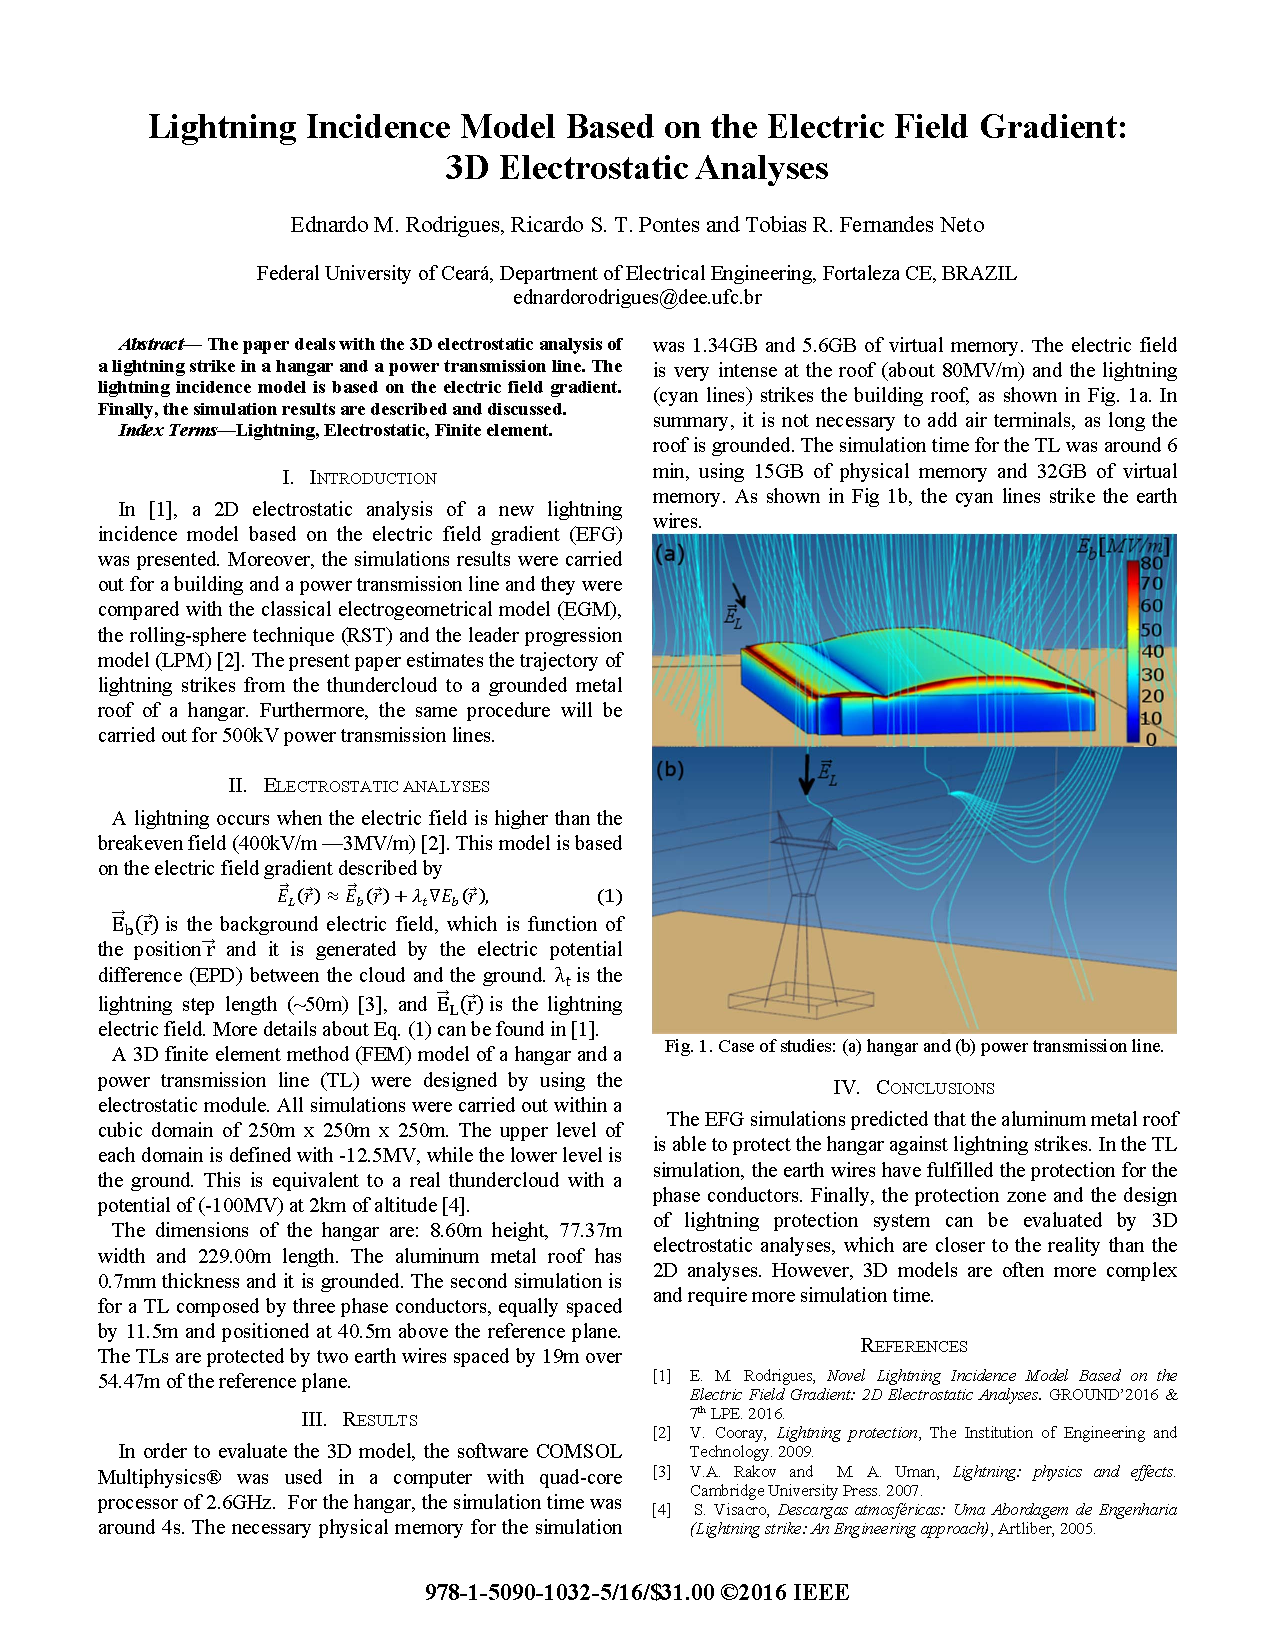
\includepdf[pages={-}]{3-pos-textuais/apendices/PID4416093.pdf}
	\imprimiranexos
		% Adicione aqui os anexos do seu trabalho
		\anexo{Ementa da Disciplina de Sistemas Eletrônicos Digitais Reconfiguráveis}
\label{an:ex_anexo_a}

Ementa da disciplina de sistemas eletrônicos digitais reconfiguráveis.

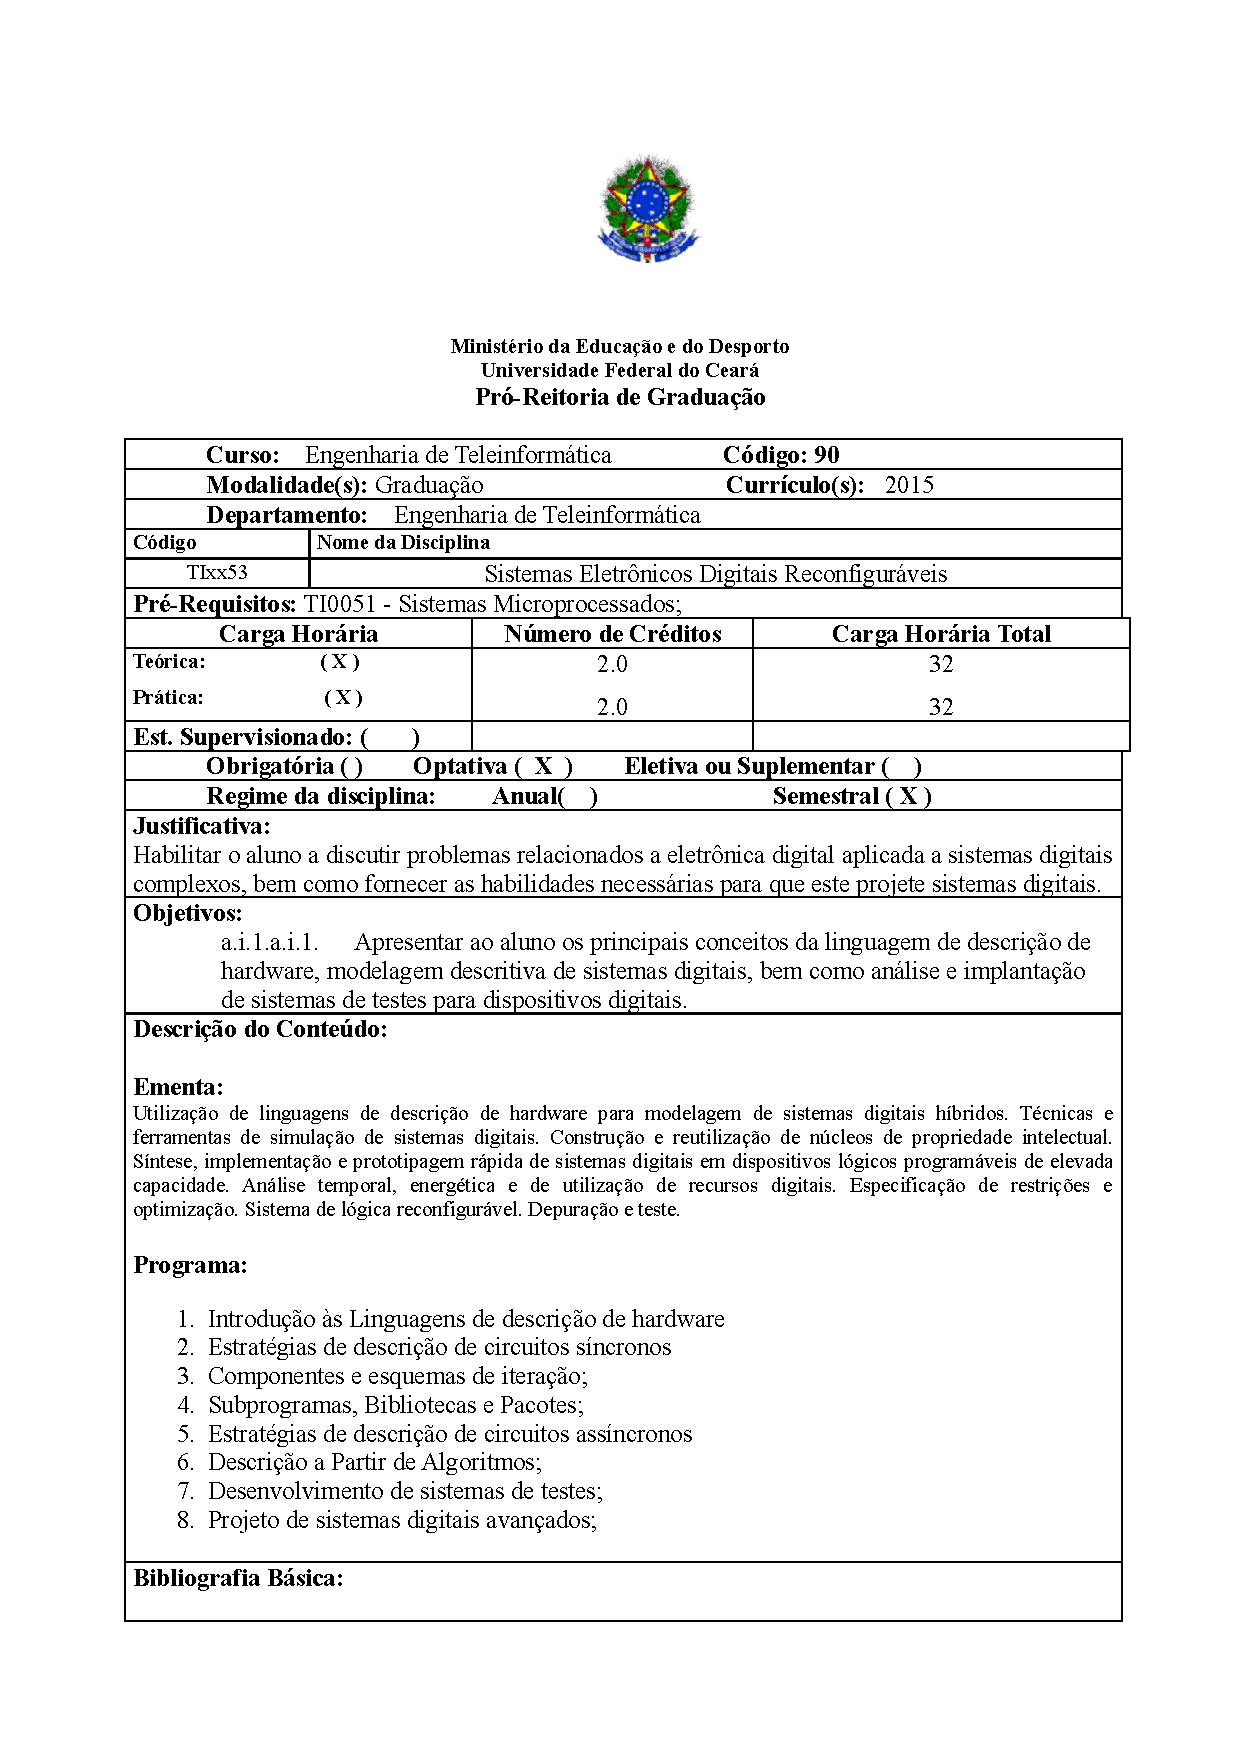
\includepdf[pages={-}]{3-pos-textuais/anexos/sistemas-eletronicos-digitais-reconfiguraveis.pdf}


		\anexo{Exemplo de um anexo em PDF}
\label{an:ex_anexo_b}

O autor pode anexar um \gls{PDF}, traduzido como formato portátil de documento. Veja o código fonte utilizado para anexar o arquivo ``Sikasil.pdf'' que foi colocado dentro da pasta ``anexos'' que por sua vez está dentro da pasta ``elementos-pos-textuais''. Tenha muita atenção na hora de especificar o local do arquivo. Recomenda-se não utilizar caracteres especiais para nomear pastas e, principalmente, arquivos. 

Pode-se fazer uma descrição sucinta do arquivo anexado.

%Comando para incluir um arquivo em PDF:
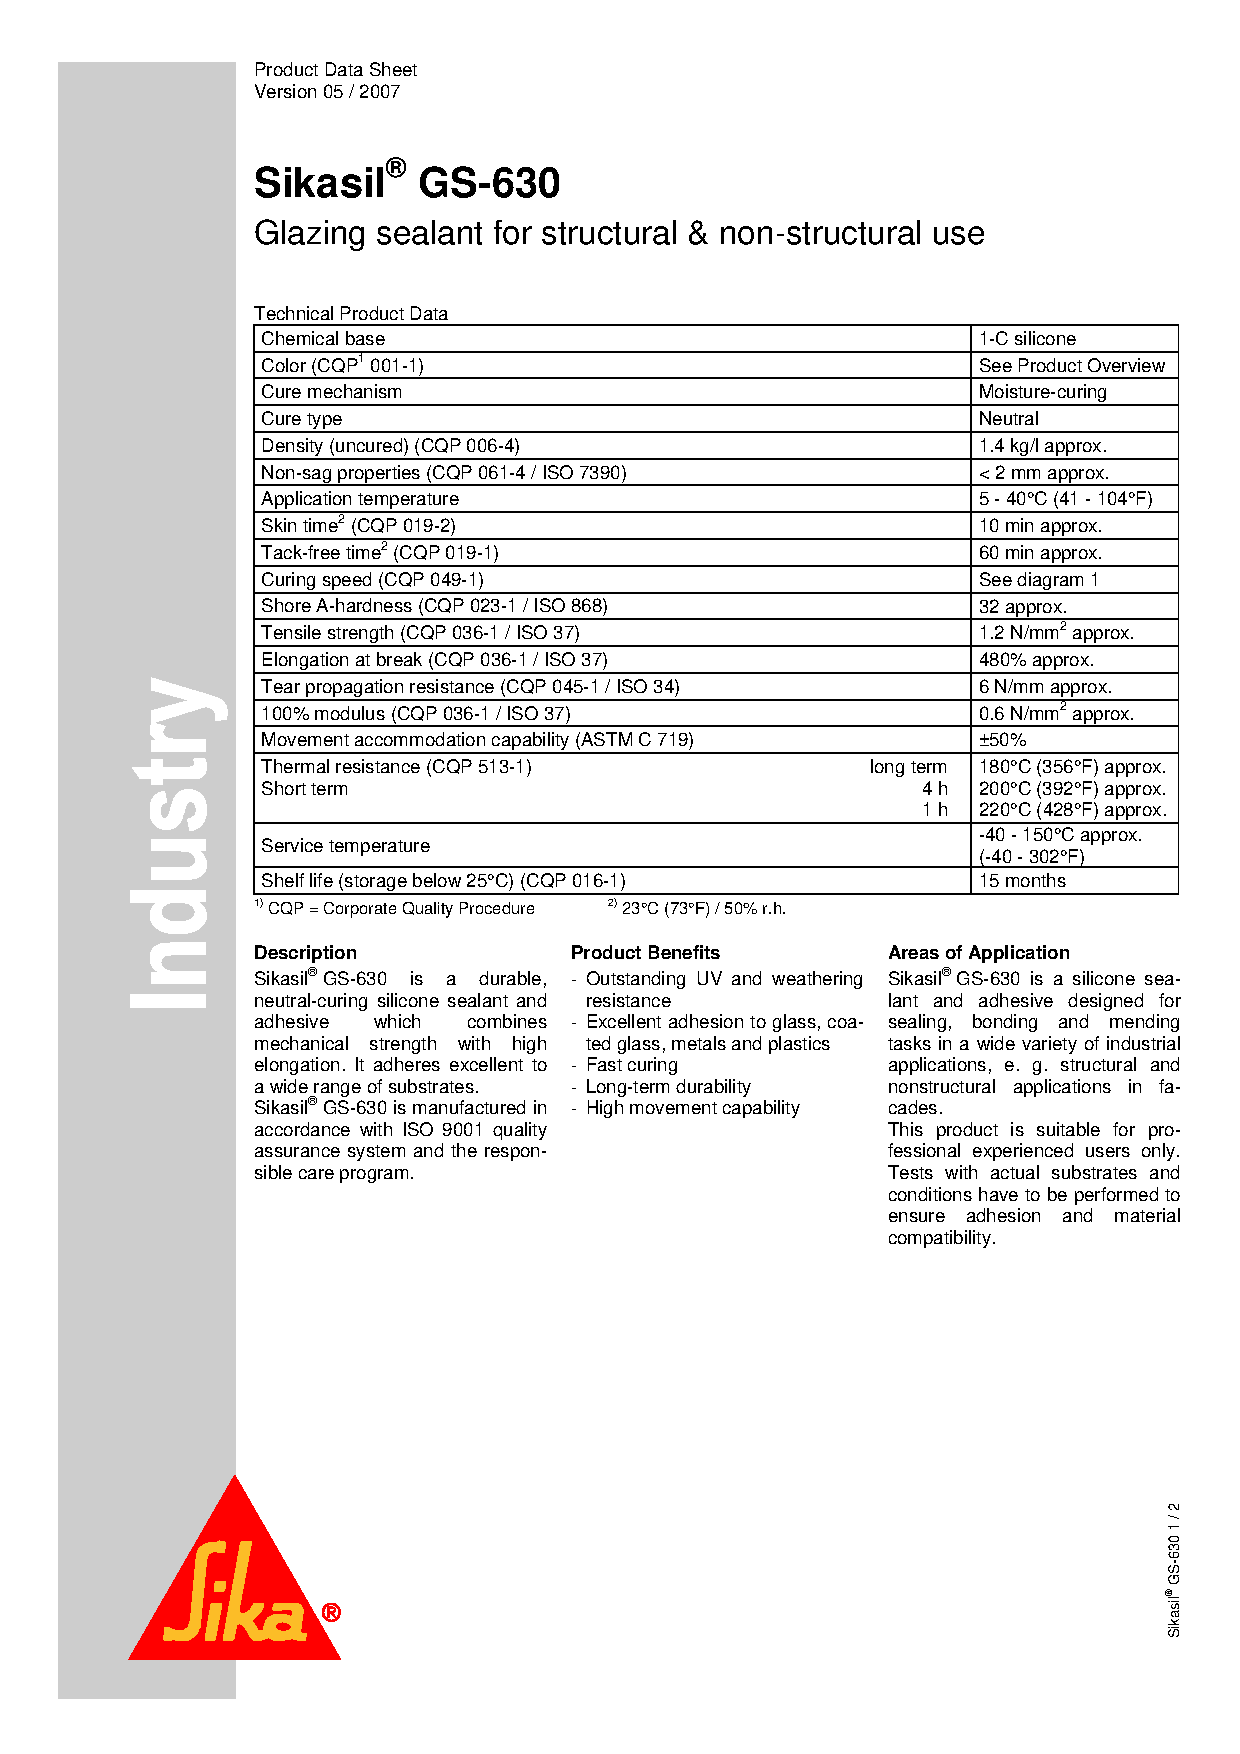
\includepdf[pages={-}]{3-pos-textuais/anexos/Sikasil.pdf}

		
	\imprimirindice

\end{document}